\documentclass[12pt]{gatech-thesis}

\usepackage{amsmath,amssymb,latexsym,float,epsfig,subfigure}

\title{A Sizing and Vehicle Matching Methodology for Boundary Layer Ingesting Propulsion Systems} %% If you want to specify a linebreak
                               %% in the thesis title, you MUST use
                               %% \protect\\ instead of \\, as \\ is a
                               %% fragile command that \MakeUpperCase
                               %% will break!
\author{Jonathan C. Gladin}
\department{School of Aerospace Engineering}


\principaladvisor{Professor Dimitri Mavris}
\committeechair{Professor Dimitri Mavris}
\firstreader{Dr. Brian Kestner}
\secondreader{Dr. Brian German}
%\setcounter{secnumdepth}{2}
\degree{Doctor of Philosophy}

%% Set \listmajortrue below, then uncomment and set this for
%% interdisciplinary PhD programs so that the title page says
%% ``[degree] in [major]'' and puts the department at the bottom of
%% the page, rather than saying ``[degree] in the [department]''

%% \major{Algorithms, Combinatorics, and Optimization} 

\copyrightyear{2015}
\submitdate{August 2015} % Must be the month and year of graduation,
                         % not thesis approval! As of 2010, this means
                         % this text must be May, August, or December
                         % followed by the year.

%% The date the last committee member signs the thesis form. Printed
%% on the approval page.
\approveddate{~~}

\bibfiles{Gladin-thesis}
\graphicspath{{../img/}}
%% The following are the defaults
%%    \titlepagetrue
%%    \signaturepagetrue
%%    \copyrightfalse
%%    \figurespagetrue
%%    \tablespagetrue
%%    \contentspagetrue
%%    \dedicationheadingfalse
%%    \bibpagetrue
%%    \thesisproposalfalse
%%    \strictmarginstrue
%%    \dissertationfalse
%%    \listmajorfalse
%%    \multivolumefalse

\begin{document}
	
	\bibliographystyle{gatech-thesis}
	
	\begin{preliminary}
	
		\begin{dedication}
\null\vfil
{\large
\begin{center}
To myself,\\\vspace{12pt}
Perry H. Disdaiful,\\\vspace{12pt}
the only person worthy of my company.
\end{center}}
\vfil\null
\end{dedication}

		\begin{abstract}
  This is the abstract that must be turned in as hard copy to the
  thesis office to meet the UMI requirements. It should \emph{not} be
  included when submitting your ETD. Comment out the abstract
  environment before submitting. It is recommended that you simply
  copy and paste the text you put in the summary environment into this
  environment. The title, your name, the page count, and your
  advisor's name will all be generated automatically.
\end{abstract}

		\begin{preface}
Theses have elements.  Isn't that nice?
\end{preface}
	
		\begin{acknowledgements}
I want to ``thank'' my committee, without whose ridiculous demands, I
would have graduated so, so, very much faster.
\end{acknowledgements}

		\contents
		
		\begin{summary}

\indent The current trend in industry standards for aviation technology is towards technologies with more fuel efficient and less noisy vehicles and power systems. One concept which has been used to much success in marine propulsion applications, and has been identified for future potential fuel burn savings for aviation is the "Boundary Layer Ingesting" (BLI) propulsion system.  This technology has been investigated at the theoretical level for aviation applications over the years by a few authors and has been the subject of extensive research in recent years in academia, industry, and government, due to the increased synergy of the concept with new vehicle designs such as the hybrid wing body.  

\indent The benefit of the BLI propulsion configuration comes from the basic fact that ingesting a portion of the aircraft upper surface tends to re-energize the low velocity boundary layer flow and thereby increase the propulsive efficiency of the system.  This, however, is counteracted by the fact that gas turbine component tend to operate with less efficiency and stability when subject to heavily distorted flow conditions.  The design challenge for BLI, then, is to maximize the amount of boundary layer which can be ingested while minimizing the negative impact of BLI on the gas turbine operation.  However, this task is made difficult due to the strong multi-disciplinary nature of the interactions between the engine and the airframe.

\indent  For the civil aviation engine designer, BLI poses a problem at the conceptual level because their are many new interaction effects where data must be filled into cycle analysis models, and such data may not be available in conceptual design.  This leaves the cycle analyst with a difficult task to quantify these effects and understand the impact of the uncertainty in the interactions on the choices made with regard to the engine cycle, the number of engines chosen, and other such conceptual level considerations.  Methods used to date have employed simple approaches for cycle analyses whereby the boundary layer is characterized using data from a single CFD solution or from closed form boundary layer approximations.  The losses are sometimes ignored, or are modeled parametrically with independent efficiency parameters in the cycle model.  Furthermore, cycle analysis methods to date have typically only employed a single design point methodology, thus ignoring the impacts of BLI at important design points like take-off, top of climb, and sea-level-static conditions and also ignoring the fact that engines often operate at different inlet conditions during flight causing a disparity in engine thrust.  Finally, conceptual level approaches typically ignore the impact of fan operability on the design trades made.

\indent The present thesis presents a conceptual level method for cycle analysis which employs multiple design conditions and multiple inlet conditions in the propulsion system sizing process.  The effects of BLI are modeled using a physics based approach, but are also modeled probabilistically so that uncertainty in the loss parameters can be mapped to the system level performance to determine the most important factors and design conditions for future development and experimentation.  A method for sizing the propulsion system in the presence of uncertainty is proposed which can provide a means for designing for additional thrust given that loss parameters may be higher than initially estimated on the real vehicle.  These methods will be tested on a hybrid wing body vehicle model with ultra hi-bypass geared turbofan engines ingesting a portion of the aircraft boundary layer.  An investigation of the effects of operability constraints on the propulsion system design space will also be tested.


\end{summary}

	\end{preliminary}

	\chapter{Introduction}

\section{Environmental Pressures and Aviation Technology}
\indent The current trend in industry standards for aviation technology is towards technologies with more fuel efficient and less noisy vehicles and power systems. Many entities including government agencies such as NASA and the FAA are interested in studying the effects of specific technologies to assess the potential return on investment of the technology to properly appropriate scarce government research dollars. In this context, many technologies require reasonable assessments of improvements at the conceptual level, when much design information is utterly lacking.  In many cases, the technologies of interest are new materials, which may simply require refinement of the manufacturing processes required to achieve the necessary material strengths and thermal properties. Other types of technologies are related to the design of specific components which improve efficiencies, decrease losses, or improve operability and durability throughout the component lifetime. Another class of technologies are those which alter the aerodynamics of the vehicle, such as winglets, ribs, or boundary layer laminar flow control. Such technologies are more dependent on the design of the vehicle and require proper design of the technologies. The environmental benefits of these technologies thus rely upon having reasonable design methods to assess their potential improvements.  One such technology which falls into the latter class and is the subject of this thesis is boundary layer ingestion, or "BLI" for short. Rather than being a "technology", it is instead a novel arrangement of the propulsion system such that it interacts positively with the aircraft wake to produce higher propulsive efficiencies. This is done by at least partially embedding the engine into the aircraft surface and ingesting the low-momentum boundary layer flow into the propulsor. Ingesting the boundary layer is beneficial because of the natural tendency for turbomachines, such as a fan, to do more work on sections of the flow with lower total inlet pressure \cite{Smith1993}.  BLI therefore has the effect of re-energizing the aircraft wake thereby reducing total drag relative to an aircraft with podded engines and improving the propulsive efficiency of the system.  NASA has identified aggressive fuel burn targets for the next generation of aircraft and beyond as shown in figure \ref{Fuel_Burn_Targets}.  Boundary layer ingestion has been identified as a potential technology to help enable the achievement of these fuel burn targets.  


\begin{table}[ht]
\caption{NASA fuel burn targets for the next generation of aviation vehicles. \cite{Kestner2011}}
\centering
\begin{tabular}{cc}
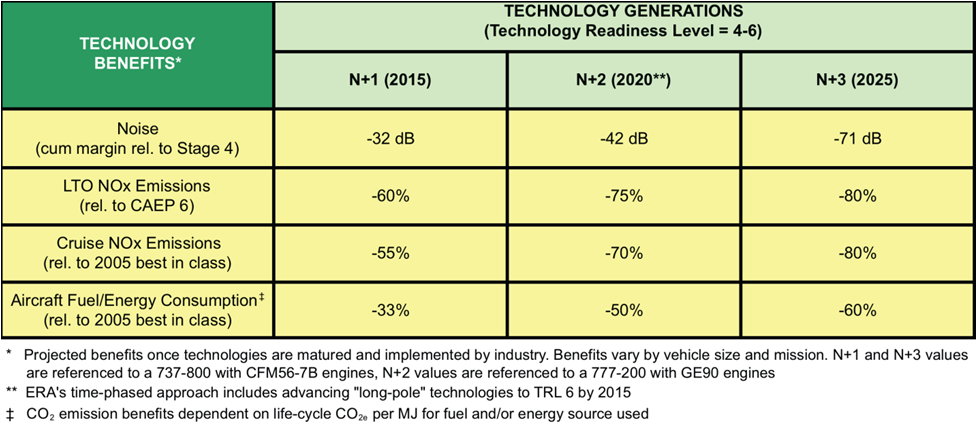
\includegraphics[width=120mm, height = 70mm, trim=0mm 0mm 0mm 0mm, clip=true]{Fuel_Burn_Targets.png}
\end{tabular}
\label{Fuel_Burn_Targets}
\end{table}


\section{Boundary Layer Ingestion}
Boundary layer ingestion (BLI) has been known and practiced within maritime engineering for quite some time now. The main effect comes from the propulsive efficiency gains from ingesting the low-momentum flow into the propulsor and re-energizing the flow to a velocity much higher than it would be otherwise, thereby reducing the overall propulsive power required to overcome the dissipative forces acting on the vehicle. In aviation, the gains from BLI are theoretically plausible and have been studied at some length but have yet to come to fruition in civil applications due to the additional difficulty of designing a proper aerodynamic intake which can deliver reasonable levels of distortion to the fan and compression system at transonic flight speeds and Reynold's numbers. However, the next generation of aircraft may have much better performance synergy with the integrated propulsive systems such that the costs of designing to negate the impacts on the engine operation of BLI are offset by the reduction in fuel consumption. One such futuristic aircraft which synergizes well with the BLI concept is the hybrid wing body. The synergy with BLI arises from the large space on the upper surface of the aircraft which is available for the placement of engines within the airframe. There are other aircraft configurations for which BLI could be a plausible option, including the "double bubble" aircraft, which is an aircraft resembling a conventional tube and wing aircraft but with a significantly flatter and wider body on the upper surface allowing for 2 or 3 embedded BLI engines. In fact, the configuration is such that almost the entire upper fuselage boundary layer can be ingested into the engine, which is a relatively large percentage of the total vehicle drag.  There are various possibilities for propulsion system configurations which may include BLI. These possibilities include but are not limited to distributed propulsion, embedded, or flush-mounted. A distributed propulsion system is a system with many small propulsors "distributed" over the upper surface in an array type configuration.  This type of system is synergistic with BLI for reasons to be explained later in this chaper. The embedded and flush mounted configurations refer to the relative position of the engine compression face centerline with respect to the inlet highlight centerline. The embedded system has an "S-Duct" which guides the flow to the engine compression system situated lower in the airframe. The "flush-mounted" system has the engine flush with the aircraft surface meaning that the wetted area of the nacelle cowl would be slightly larger than the embedded case.  Among these configurations, there are multiple engine architectures which are possible including traditional turbofan direct-drive engines, geared turbofans, single-core/multi-fan type systems (e.g. tri-fan).  The single-core/multi-fan type systems have the benefit of being able to ingest much more boundary layer while avoiding the negative impacts on the gas turbine core.  Any design method for BLI systems must be able to include the physical performance differences between these engine congurations as well as the system weight and mission analysis to determine fuel burn for the entire system.

\subsection{BLI Benefits}
The benefits of BLI can be described, in principle, as a reduction in the total power requirement of the vehicle due to the increase in propulsive efficiency.  Additionally, the weight of the propulsion system is typically improved because of the elimination of the need for an engine pylon. There is also a nacelle wetted area reduction since the pylon and nacelle wetted area is less with the embedded or flush mounted engines having some of their surface area contained within the aircraft and not wetted by the air.  Lowering the engine closer to the airframe also incidentally has the effect of improving the pitch control of the aircraft with the thrust vector momentum arm being smaller.  

\indent Figure \ref{Podded_vs_Embedded_Engines} illustrates the basic difference between an ideal BLI engine and a podded engine \cite{PlasThesis}.  Here U$_\infty$ represents the free-stream velocity and $U_w$ represents the averaged wake velocity in the podded case. From classical propulsion theory, the input power required is given by equation \ref{Power_Added_Podded} for the podded case and by equation \ref{Power_Added_BLI} for the BLI case, where Uj is the jet velocity exiting the nozzle and is assumed to be the free-stream velocity in the BLI case.
    \begin{figure}
    \centering
    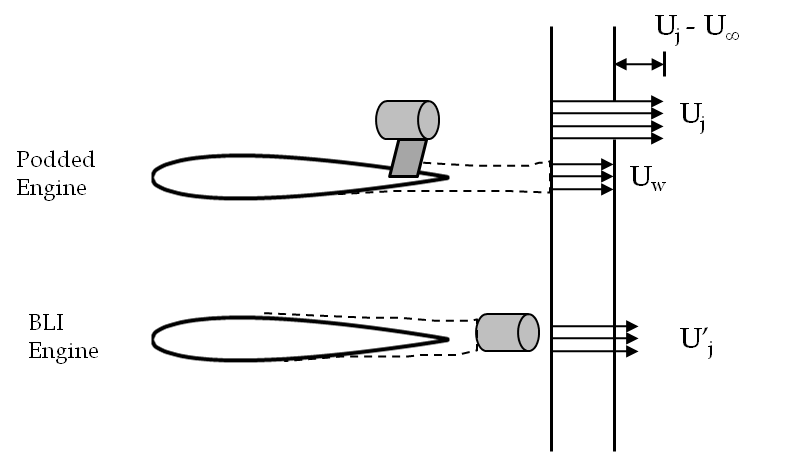
\includegraphics[width=140mm, height = 80mm, trim=0mm 0mm 0mm 0mm, clip=true]{Figure1_Podded_vs_Embedded_Engines.png}
    \caption{Notional diagram of podded vs. BLI engine design}
    \label{Podded_vs_Embedded_Engines}
    \end{figure}
\begin{equation}P_{Podded}= \frac{\dot{m}}{2}\big(U_j^2-U_\infty^2\big) = \frac{F_{n Podded}}{2}\big(U_j+U_\infty\big)\label{Power_Added_Podded}\end{equation}
\begin{equation}F_{n Podded}= \dot{m}\big(U_j-U_\infty\big) \label{Net_Thrust_Podded}\end{equation}
\begin{equation}P_{BLI}= \frac{\dot{m}}{2}\big(U_j^2-U_w^2\big) = \frac{F_{n BLI}}{2}\big(U_j +U_w\big)\label{Power_Added_BLI}\end{equation}
\begin{equation}F_{n BLI}= \dot{m}\big(U_j-U_w\big) \label{Net_Thrust_BLI}\end{equation}
Since $U_w$ is inherently less than the jet velocity, comparing equations \ref{Power_Added_Podded} and \ref{Power_Added_BLI} shows that the power required for the BLI case is less than for the podded case.  Although this is the simplest idealization of BLI, this is sufficient to explain the basic physics.  Because of the aero-propulsion interaction, the total benefit of the system is dependent on the propulsion system arrangement and the incoming airframe wake at the intake location, thus leading to the large disparity in possible benefit. 
\subsection{BLI Risks}

Perhaps the most significant risk with regard to BLI is the performance of the inlet and fan system.  The intake of an aircraft engine, while simple, is an absolutely essential component whose performance has a high impact on the specific fuel consumption of the engine.  The intake must supply the necessary amount of air flow to the compression system to accomodate the required level of thrust without significant losses or flow distortion which can lead to performance degradation or compression stability concerns. Two risks arise from this problem: 1.) inherent uncertainty in engine performance (related to inlet total pressure recovery and fan distortion); 2.) Compromised stability of the compression system due to the presence of both steady-state and dynamic inlet total pressure and swirl distortion.  In other words, there is a risk that the BLI induced gains in propulsive efficiency may be offset by the presence of a poorly performing inlet configuration and also risk that the engine, while more efficient, might simply not be operable over the required flight envelope of a civil air transport. Nichols, in an evaluation of the Silent Aircraft Initiative, also identifies these risks as the primary factors of uncertainty for the concept.  

There are other ancillary risks such as the effect of the distortion on component degradation and lifetime. Such factors can significantly impact operability costs and potentially offset some of the fuel burn cost savings. There is also the additional difficulty of designing a system which has a highly integrated airframe and propulsion system. This concern is exacerbated by the fact that these components are produced by separate companies requiring the need for intercorporate cooperation to certify this new technology and provide for an economical design. There are also other detailed factors such as the control of a system which is specifically designed to have steady-state and transient turbulent distortion present during operation or vibration which might arise from the same phenomenon. Significant research funding has gone into investigating the possibility of designing a "distortion tolerant fan" which can operate under the types of distortion related to BLI with improved efficiency and stall margin. However, this possibility remains uncertain as the research is still in progress.

\section{Design Methods}
Before talking about the methods of engine design with BLI, it is worth discussing some general design terminology and concepts. Broadly speaking, there are 3 primary phases of the design process: conceptual, preliminary, and detailed. The conceptual design phase is the very earliest phase in which system requirements, architecture, and basic performance characteristics are formulated. Preliminary design moves the system towards a more concrete physical definition by giving some of the components geometric definition, and initial conceptual performance estimates are modified in light of the new design information. Detail design is logically the next phase in which every single detail of the design is decided up to the point where manufacturing takes place. This last phase is the most involved, most expensive, and therefore the most costly should errors in the process necessitate design changes. Recent advances in design over the course of the last few decades have transitioned towards including elements of the latter two design phases in the conceptual phase using higher-order physics based tools to estimate detailed design performance. This is really happening because some of the newer technological concepts require detailed design understanding and quantification in order to determine the feasibility of the technology up front.  BLI is certainly a great example of where this design paradigm is most appropriate, since the propulsion design essentially depends upon the characteristic of the engine intake and the thrust requirement coming from the vehicle aerodynamics and flight conditions, thus lending itself to higher fidelity multi-disciplinary methods.  Conceptual design is the most important phase in the design process, especially for complicated systems with many subsystems.  Early design mistakes due to large uncertainty in performance or system feasibility can have large influence on costs later in the design phases, since all component designs depend on conceptual design choices. As such, changes in the conceptual  design of the system can have critical consequences if made in the detail phase and are amplified as the product matures.  

In the case of newer technologies which are unproven and highly uncertain, the need to minimize uncertainty and maximize the probability of success of the technology when integrated into a system is especially high. This can be difficult since technologies are not only expected to be able to maintain current state of the art capability but to improve upon it substantially to justify the additional research expenditures and investment involved in it's development.  Potential customers need to know that the product will be as reliable as their current technology but will offer additional operability cost savings to justify new purchases. If the technology benefits are not proven to customers or are shown to be negative, then the aircraft program could stand to be cancelled leading to large lost cost.  


\subsection{Conceptual Architectural Studies}
There are a number of conceptual design methods for propulsion systems in use today. The most common, at least at the conceptual level, is the thermodynamic cycle analysis. Typically these are "0-D", axisymmetric analyses that aim to provide thermodynamic gas path properties, thrust, and fuel flow. This type of analysis typically requires some characterization of each component of the propulsion system (from compression systems to the intake, nozzles, ducts, and combustors).  Cycle analysis is done in two modes: on-design and off-design. In on-design, the engine is sized to meet specific thrust targets at a given flight condition(s). In off-design, the performance of the engine is determined at other ambient conditions that are not considered the design condition. The final product of this analysis is engine thrust and fuel flow as a function of mach number, altitude, and throttle (power code). This is typically called the "engine deck". This information is used in the aircraft sizing and synthesis analysis to determine total take-off gross weight and mission fuel burn. In this way, changes in engine design or technology can be mapped to the system level through physical analysis.  Recent advances in cycle modeling tools have made "multiple-design point" on-design cycle analysis possible. This is the process of simultaneously satisfying multiple thrust targets and constraints at various conditions, whereas traditional single-point design only considers one. This is necessary because propulsion systems need to satisfy thrust requirements at various flight conditions such as top of climb (TOC), cruise, take-off (TKO), and sea-level static (SLS). Many studies focusing on BLI tend to only include the cruise or SLS conditions as the thrust sizing points when doing the on-design cycle analysis, which is really inadequate. More details will be given in chapter 2 on the MDP cycle analysis process and how it might be used with BLI.  For BLI, there have been many studies which involve the use of cycle analysis, even though modeling BLI requires some way of representing the non-uniform flow.  One way of doing this is to simply mix (average) the flow. This leads to certain errors in performance estimates since averaging the flow in this way tends to violate one conservation law or the other (mass, momentum). There are other methods of modeling the impact of BLI on cycle performance which resolve this difficulty such as the parallel compressor model, which is a "1-D" analysis and tends to better capture the impact on fan efficiency and stall margin. More complicated methods can also
predict the distortion transfer across the fan which can have an impact on the final performance.  Many of the studies that have implemented these types of 0-D or 1-D analyses are intended to give a first order estimate of fuel burn benefit. These estimates are used for architectural trade studies to determine the number of engines, engine placement, engine cycle, and other engine parameters. Typically higher order analyses are required for determining the detailed design of the inlet and external cowl shape, but such analyses require a cycle model to create boundary conditions for the computational analysis. A parametric cycle model also allows up-front sensitivity studies on the CFD analysis results.

\subsection{High-Fidelity Integration Studies}

There is another basic type of study which is common in the BLI literature which relate more to the detailed design of the inlet configuration. These are typically done to design the shape of the inlet diffuser and external cowl based on computational fluid dynamics. The objective of these are to reduce inlet distortion and total pressure loss, and to get better estimates of the total drag of the vehicle with the integrated engine.  These details are very important to the quality and performance of the design, but are additionally very expensive to obtain because BLI requires some level of viscous analysis (typically RANS) and is subject to separation effects which can require very refined grid sizes. Higher order studies tend to be more computationally expensive than the simpler 0-D or 1-D estimates which means that the designer should have aviable choice of propulsion system architecture and engine cycle before going to the detailed higher-fidelity phase. Spending limited computational resources on shape optimizing an inlet for a sub-optimal configuration is obviously undesirable.

\section{Need for a Propulsion Systems Design Framework}

\indent As such, the design process must involve designing to maximize the influences of the benefits and reduce the influence of the risks as economically as possible. In the case of BLI propulsion systems, this requires appropriate choice of architecture, component designs, engine type, and many other factors all of which affect the technology "benefit". BLI surely offers a design benefit in theory, but its presence is so physically significant that it necessitates changes in the way that the engine and airframe are designed to ensure system viability. It is not simply something that can be added to any design and be expected to yield a high confidence benefit, which is part of what makes this a challenging and interesting problem.
\indent A recent report by Boeing and NASA state that the BLI technology is currently "TRL 2" \cite{Bradley2012}.  Technology readiness level, or TRL, is a qualitative measure of how ready or proven a given technology is for practical usage.  The study states that the current state of the technology includes \cite{Bradley2012}:
\begin{itemize}
\item{Concepts for reducing distortion have been studied.}
\item{Some BLI configurations have been conceived.}
\item{Some studies have shown benefits for BLI.}
\end{itemize}

To mature the technology to TRL 3, the maturation plan for BLI is stated as:

\begin{itemize}
\item{A conceptual BLI aircraft configuration will be developed as a focal point for more detailed
development and as target for assessment of system-level benefits.}
\item{A BLI engine installation will be designed and analyzed with goals of ingesting substantial
boundary layer flow while keeping the boundary layer flow away from the engine core.}
\item{Approaches for reducing distortion from ingested boundary layer flows will be analyzed.}
\item{The BLI aircraft aerodynamic lines will be adjusted for the BLI engine installation.}
\item{Aerodynamic analysis of the integrated BLI configuration will be performed for cruise and
significant off-design conditions.}
\item{BLI-compatible engines will be designed for best efficiency given the anticipated engine flows.}
\item{A concept for BLI engine structural integration will be developed and analyzed.}
\item{A system-level assessment of the benefits of BLI will be made from the results of the analysis
studies.}
\end{itemize}

Note that the second bullet in the above list is the selection of a BLI installation for ingesting maximum boundary layer.  The following bullets then discuss the potential tactics for battling the inlet distortion, improving aerodynamic efficiency, and finally designing an engine which maximizes efficiency given the aerodynamics of the configuration.  The problem with this design process is that the initial analysis which determines the BLI engine installation will need to account for some of the information which is to be defined in later steps.  This provides the basic motivation for a conceptual, physics based, system level analysis tool which can account for uncertainty in the inputs to the system level model.  As such, the primary research objective for this dissertation is as follows:

\vspace{25pt}
\fbox{
  \parbox{\textwidth}{Primary Research Objective:  Develop a methodology for conceptual system level analysis of BLI propulsion systems which can allow for simultaneous satisfaction of system requirements and constraints at multiple design conditions, quantify BLI performance impacts, determine critical design conditions, and quantify sources of uncertainty and their relative contribution to variation in the system metrics of interest and select a design which is robust to uncertainty.  
}
}


	\chapter{Literature Review}

\section{Boundary Layer Ingestion Models}

There are various approaches for modeling the effect of boundary layer ingestion on an aircraft.  The primary differences between these methods is the fidelity of the models and the design capabilities that they allow.  Some of the simpler models have basic, conceptual level parameters which define inputs to the model and with which the designer can understand the relevant trends.  Higher order methods tend to be less parametric and require much more computational time, and for that reason are typically reserved for the later stages of design where detailed design features need to be set, and the uncertainty in the result must be inherently lower.  Since this thesis work focuses on engine design at the very earliest conceptual stages in the context of BLI, the focus of this chapter is to outline some of the major approaches that have been taken to model BLI at the conceptual level.  The purpose of this chapter is to outline the basic theory of each of these models, summarize the results from previous studies which employed them, and to assess the relative short-comings and benefits of each of them to provide a basis for later model selection and adaptation.  Additionally, this chapter will substantiate the need for the current work by outlining the overall shortcomings of previous approaches to identify areas of improvement in both modeling and design methodology.

\section{Boundary Layer Ingestion Literature Review}
\subsection{Classic Studies}
Boundary layer ingestion really stems from considerable usage in marine propulsion where it is much easier to take advantage of the large ship wake that can be ingested by an aft mounted propeller.  It has been researched somewhat in previous investigations for aircraft applications however.  The first investigation of BLI was conducted by A.M.O. Smith \cite{Smith1947}.  In 1946, Smith conducted an analysis of a turbojet engine and aircraft design with standard inlets and with BLI inlets. The BLI inlets were idealized as slots installed over the wing.  Smith showed a 30\% improvement in fuel efficiency and a 7\% higher optimum cruise speed, though this is in comparison to designs of the time.

Lynch \cite{Lynch1960} performed a momentum analysis on an early turbofan engine design that ingested fuselage boundary layer and obtained a 3\% improvement in propulsive efficiency accompanied by a 6-10\% decrease in maximum engine thrust. Lynch’s analysis also depended on the assumption of minimal inlet losses.

Douglass \cite{Douglass1970} performed an energy wake analysis on an aircraft with aft fuselage-mounted engines. The engines were assumed close enough to the fuselage to ingest the boundary layer. Douglass’ analysis suggests up to a 10\% improvement in propulsive efficiency compared to an equivalent pylon mounted engine installation. 

\subsection{Recent System Studies}
There has been a significant amount of research conducted on the BLI concept in essentially the last decade.  This work has focused on many different vehicle concepts as well as many different aspects of the problem ranging from system level trade studies and technology risk assessment to high-order computational analyses and optimization of inlets and nacelles.  There have also been some funded experimental studies, leaving at least a small amount of experimental data for certain designs -- most commonly the inlet and fan.  This thesis pertains to system studies at the conceptual level and so the following section will summarize in some detail the goals, general modeling approach, and conclusions of recent system level studies as well as show a comparison of the high level benefit for each of the identified studies.  

\subsubsection{Boeing Studies}
Dagget et. al. conducted a study for the Boeing company under the Ultra Efficient Engine Technology/Propulsion Airframe Integration Project.  The study was designed to analyze the effect of BLI on the BWB aircraft with active flow control (AFC).  The engine analysis was done using the "ram drag" approach, meaning that the ram drag term contained within the net thrust is reduced by a percentage which is calculated based upon the boundary layer characteristic averaged over its height.  The analysis included 3 tasks:  first the establishment of a baseline; second, the evaluation of embedded engines with BLI; third, evaluation of active flow control (AFC) to inlets.  A podded engine based off of typical engine technology was established as the baseline engine.  For the BLI configuration, a long S-Duct, highly off-set embedded inlet was used to establish the fuel burn benefits from the ram drag reduction.  It was determined that the baseline BLI configuration would offer 3.1\% fuel burn improvement, which is relatively substantial.  With the addition of the AFC technology, the inlet duct can be shortened which has weight, wetted area, and total engine length benefits.  This also allows the use of high aspect ratio inlets which allows for larger ingested boundary layer.  The fuel burn benefit with the AFC technology and the shorter low-offset inlets was estimated as 5.5\%.  

\indent Another study conducted by the Boeing company focused on the inlet configuration and the potential benefits offered by increasing the aspect ratio of the inlet.  The approach and general vehicle configuration was very similar to that studied in ref. XX.  The study also refined the calculation for the nacelle viscous drag by "proper analyses of viscous changes where reductions in nacelle drag account for local Reynolds Number effects".  This accounting difference led to a much greater estimate of the potential of BLI with AFC and flush mounted inlets which was estimated at ~10\% maximum.  It was determined that the lower aspect ratio inlet (higher height than width) resulted in a better net fuel burn than the larger width inlets due to the fact that the inlet pressure recovery was assumed to be 1\% different.  The result of this is therefore dependent on the validity of this assumption.  If the lower and wider inlet (higher AR) can be kept at sufficiently similar levels of inlet recovery, it should offer larger benefit due to the increased amount of drag ingestion and improved ram drag effect.

\subsubsection{Nickols}

\indent Nickols and McCullers conducted a configuration system study for the Hybrid Wing Body concept.  This study was a relatively low fidelity study which did not truly employ engine design techniques or cycle analysis.  Instead the study assumed a certain percentage drag reduction to be applied to the aircraft drag polar within the mission analysis, as well as a nacelle wetted area reduction factor, pylon weight sturctural factor, and SFC penalty due to the lower inlet pressure recovery.  The final analysis showed an impact of 5.2\% fuel burn benefit for the BLI technology.

\subsubsection{Rodriguez}
\indent Rodriguez, as a part of his doctoral work, developed a method for multi-disciplinary inlet optimization which combined high fidelity CFD methods with a propulsion model.  The method was applied to the BWB vehicle with 3 boundary layer ingesting high-bypass ratio engines.  The method consisted of optimizing the inlet and external cowl shape such that the fuel burn rate is minimized while maintaining an acceptable level of inlet distortion.  The method itself did show significant improvement from the baseline design, which highlights the importance of higher-order methods in the detail aerodynamic design phase.  However, the work showed that the same optimization applied to the podded case yielded the result that BLI did not provide any benefit (BLI was actually worse, in fact).  This could have resulted from the fact that there were a limited number of design variables for the outboard engines, yielding excess and potentially removable wave drag from the outboard engines.  Furthermore, the inlet pressure recovery was very low in comparison to recent studies which have shown potentially much higher values of inlet recovery using other optimization methods.

\subsubsection{Plas}
\indent As part of NASA's silent aircraft initiative, Plas conducted a study of boundary layer ingesting engines in which the following 3 contributions were intended:  Creation of a conceptual and theoretical framework for BLI in aircraft design; development of high fidelity models for representing an aircraft with BLI embedded engines; Quantification of the benefits of BLI.  This work is the first of it's kind that actually analyzes the impacts of BLI while including an actual model of the turbomachinery operating in non-uniform flow.  The study assumed that the configuration of interest was a ducted fan type.  The work included an assessment of three different degrees of fidelity within the fan modeling:  a one-dimensional parallel compressor approach, an integral boundary layer approach, and a 3-D body force model.  The highest fidelity of these approaches showed that BLI for the aircraft under consideration in the silent aircraft initiative gave power savings between 3-4\%.  The study also concluded that a principal feature required to estimate power saving for the propulsor is the distortion transfer across the fan (i.e. level of distortion downstream of the fan).  It was also found that the power savings differed by 10-40\% between the different fidelity fan models, although the trends remained roughly the same regardless of the modeling fidelity.

\subsubsection{NASA and UTRC}
\indent Hardin et. al conducted an aircraft system study of a BLI propulsion configuration.  The analysis included a detailed cycle model for an ultra-high-bypass propulsion system with BLI.  The system study employed lower order models for the different components of the BLI problem, including the BLI theoretical benefits; nacelle weight and drag; fan performance; and inlet pressure losses.  Aircraft trade factors were used to estimate fuel burn based on the engine cycle calculations and weight estimates, and the results of the study showed that a 3-5\% BLI fuel burn benefit could be achieved for the "N+2" generation aircraft relative to a pylon mounted baseline.  Another key conclusion was that the inlet pressure recovery and fan efficiency have a strong impact on the level of fuel burn achieved with 1\% pressure recovery loss translating to 3\% fuel burn increase.  This provides the motivation for low loss inlets and distortion tolerant fan configurations to maximize the potential benefit of the technology.

\subsubsection{Summary}
\indent A few trends arise from an analysis of the system study literature:

%%
\begin{figure}[hptb]
\centering
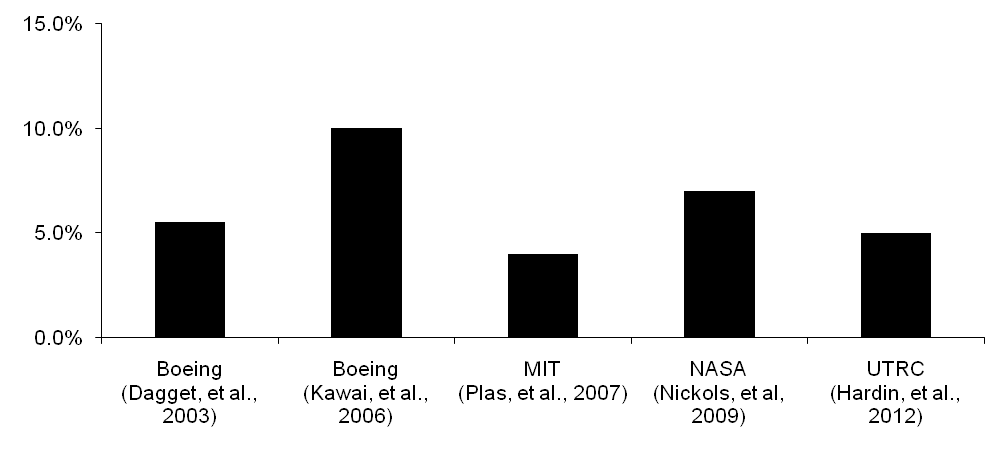
\includegraphics[width=120mm, height =60mm]{Figure4_System_Study_Estimates.png}
\caption{Boundary layer ingestion system study estimates}
\label{System_Estimates}
\end{figure}
%%

\begin{itemize}
\item{The fuel burn analysis for BLI is a function of the trade-offs between propulsive efficiency gains obtained via drag ingestion, thermal efficiency penalty due to distorted inlet flow, propulsive efficiency changes due to changes in nacelle and interference drag, and the effect on the engine and support structure weight -- all of which affect the aircraft fuel burn.}
\item{There is a wide uncertainty on the potential benefit that BLI offers for the HWB aircraft, typically ranging from 0-10\%. (See fig. \ref{System_Estimates})}
\item{The quality of the inlet, level of inlet distortion, and impact on the fan efficiency have a strong impact on the potential benefits.  This is shown by simple cycle analysis results, as well as by the study of Rodriguez, which predicted no benefit for BLI with very high loss inlets relative to studies with much improved assumptions.}
\item{Configurations which can reasonably ingest more boundary layer across the upper surface of the aircraft stand to offer larger potential benefits.}
\end{itemize}

\section{Modeling Requirements for BLI}
The boundary layer ingestion problem can be broken down into two areas with regard to performance:  propulsive efficiency improvement (BLI effect) and thermal efficiency degradation.  This is the basic trade-off upon which the economic viability of the system depends.  This is an almost trivial statement, since of course the overall efficiency of the engine is ultimately a product of the thermal and propulsive efficiencies.  However, the thing that makes the BLI problem interesting at the conceptual level is that the negative (thermal) efficiency impacts and the positive (propulsive) efficiency impacts are both functions of how much boundary layer (distorted flow) enters the engines.  As more drag is ingested into the engine, the propulsive efficiency benefits increase, however the level of distortion and general total pressure recovery decreases which impacts the performance of the propulsor and potentially the gas turbine core.  The design challenge then, stated clearly, is to maximize the amount of drag ingested while maintaining sufficiently low levels of distortion and total pressure loss such that the benefits of the propulsive efficiency gain are not prohibitive.  
\begin{figure}[htpb]
\centering
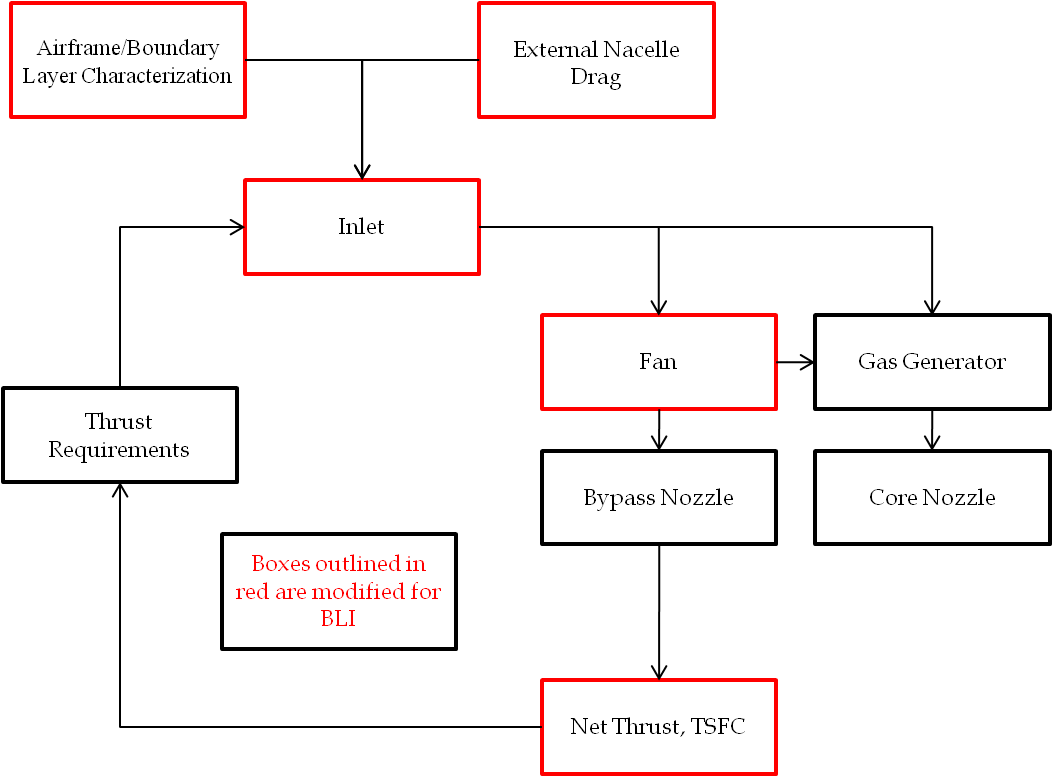
\includegraphics[width=140mm, height =80mm, trim=0mm 0mm 0mm 0mm, clip=true]{Figure2_Cycle_Analysis_with_BLI.png}
\caption{Notional cycle analysis for a BLI propulsion system.  Boxes outlined in red show the components which need modification for BLI.}
\label{BLI_changes}
\end{figure}
To do this, the designer must have proper modeling fidelity for each of the components which are impacted by the ingestion.  Design trades would then emerge from the combination of the various impacts on each component via typical cycle analysis techniques.  Fig. \ref{BLI_changes} shows the components which require modification or addition for BLI.  These are the most basic components that require modeling, however there can be other effects which impact system performance.  These include but are not limited to: impact on bypass nozzle gross thrust coefficient; impact on propulsion system weight relative to equivalent podded case; compression system stability (fan or core stall).
	The rest of the chapter will focus on describing the state of the art system level approaches taken for each of the above components which require BLI impact modeling.  Some space will also be taken to describe cycle analysis methodology, and also uncertainty and risk modeling within these systems.   

\section{General Boundary Layer Definitions and Terminology}
It is necessary to begin with a small introduction to the theoretical notion of a boundary layer and to specify some of the parameters associated with them in order to understand the review of the previous literature as many of these ideas and terms are consistently used throughout.  The concept of a boundary layer is simply a region in a flow which is affected by the presence of a nearby wall shear stress which is acting to retard the fluid.  This tends to create some velocity distribution ranging from some slow value (typically modeled as zero) at the wall to the value at the edge of the boundary layer which is typically denoted as $u_e$.  Figure \ref{Flat_Plate} shows an example boundary layer profile on a flat plate.  The thickness of the boundary layer, typically denoted as $\delta$, grows as the distance along the flat plate increases.  The non-dimensional parameter which is typically correlated with this phenomena is called the "Reynold's Number" or $R_e$ and is given by equation \ref{Reynolds}.  
\begin{equation} Re = \frac{{\rho_\infty} u_\infty c}{\mu_\infty}\label{Reynolds}\end{equation}
Where $\rho$ is the freestream density, $u_\infty$ is the freestream velocity, and c is a characteristic length.  This is the basic non-dimensional scaling parameter for viscous flow and represents the ratio of inertial forces to viscous forces within the fluid.  
%%
\begin{figure}[htpb]
\centering
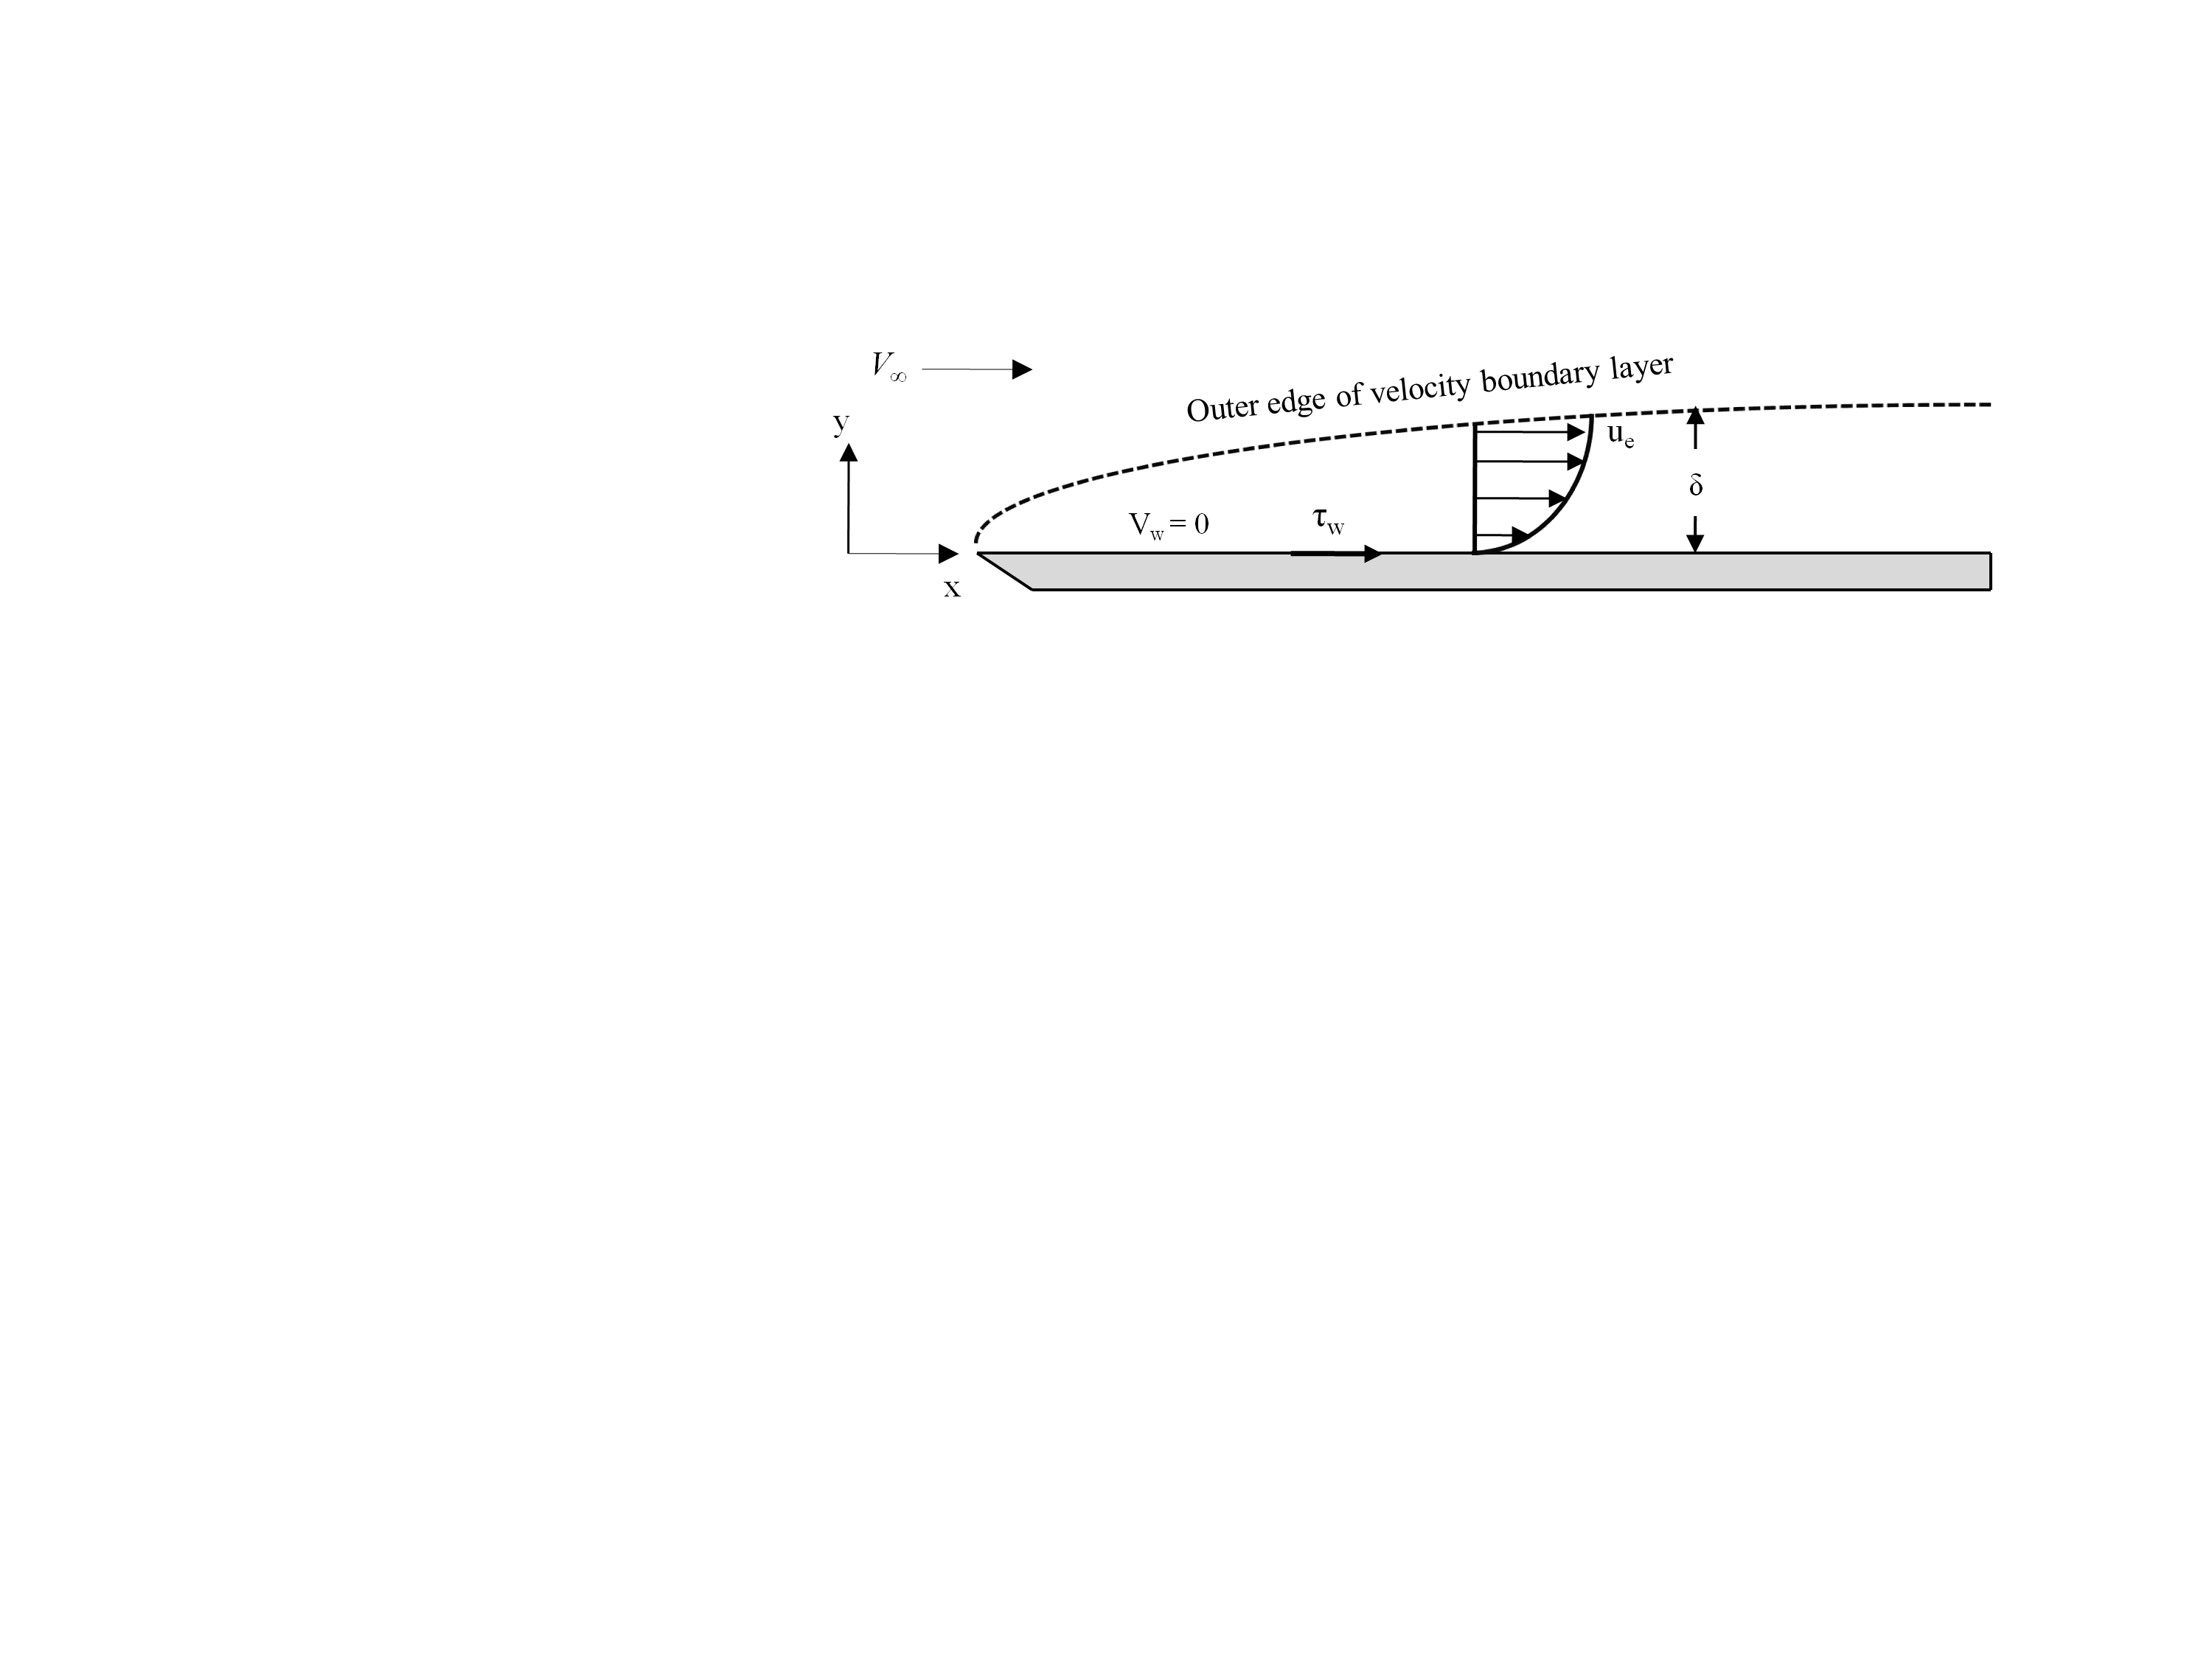
\includegraphics[width=180mm, height =35mm, trim=90mm 120mm 0mm 35mm, clip=true]{Figure3_flat_plate_BL.png}
\caption{Notional figure of a boundary layer growing on a flat plate in an aerodynamic flow.}
\label{Flat_Plate}
\end{figure}
%%
As the characteristic length increases, the size of the boundary layer thickness grows.  At the walls, the velocity is zero and the shear stress is present due to the velocity gradient and is given by equation \ref{tau_wall}.  The non-dimensional coefficient associated with the wall-friction shear stress is the skin friction coefficient and is given by equation \ref{skin_friction}.   The $\tau_w$ is a function of the distance along the x-axis since the boundary layer shape is changing and thus the gradient at the wall is changing as well.
% 
\begin{equation} \tau_w = \mu \left(\frac{\partial u}{\partial y}\right)_w\label{tau_wall}\end{equation}
\begin{equation} C_f = \frac{\tau_w}{\frac{1}{2}\rho u_e^2}\label{skin_friction}\end{equation}
%
A property commonly used to describe the boundary layer is the displacement thickness $\delta^*$ which is a measurement of the missing mass flow.  This is derived in the simple 2-D case illustrated in figure \ref{Flat_Plate} in \cite{Anderson2001}. Equation \ref{delta_star} gives an expression for the displacement thickness.  This represents the height of a theoretical stream tube, which, at the same density and velocity as the boundary layer edge, would have the same mass flow as that which is missing from the flow due to the presence of the boundary layer \cite{Anderson2001}.
\begin{equation}\delta^* = \int_0^{y_e} \left(1-\frac{\rho u}{\rho_e u_e}\right)dy\label{delta_star}\end{equation}
Another boundary layer property of importance is the momentum thickness, which is similar to the displacement thickness except that it represents the decrement in momentum in the flow due to the presence of the boundary layer.  The equation for the momentum thickness is given by equation \ref{momentum_thickness}.  The kinetic energy thickness can also be defined similarly, and represents the decrement of kinetic energy in the 
\begin{equation}\theta = \int_0^{y_e} \frac{\rho u}{\rho_e u_e}\left(1-\frac{u}{u_e}\right)dy\label{momentum_thickness}\end{equation}
\begin{equation}\theta^* = \int_0^{y_e} \frac{\rho u}{\rho_e u_e}\left(1-\left(\frac{u}{u_e}\right)^2\right)dy\end{equation}
flow due to the boundary layer dissipation.  Note that these are here defined as the 1-dimensional integral along the vertical axis.  The capital greek symbols for each of these boundary layer factors will be defined as the 2-D equivalent integrated over a surface, such as the surface area of an ingested streamtube for a BLI propulsor.  The ratio of the various factors just defined are also key indicators of the shape of the boundary layer.  These include H, $H^*$, which are defined by equations \ref{shape_factor}-\ref{pseudo_energy_factor} and the ratio of the boundary layer thickness to the displacement thickness.  Having these definitions, the Reynold's number based on the momentum thickness of the boundary layer can be defined as in equation \ref{reynolds_theta}.
\begin{equation} H = \frac{\delta^*}{\theta}\label{shape_factor}\end{equation} 
\begin{equation} H^* = \frac{\theta^*}{\theta}\label{pseudo_energy_factor}\end{equation}
\begin{equation} Re_\theta =  \frac{u_e\theta}{\nu}\label{reynolds_theta}\ref{reynolds_theta}\end{equation}
Finally, one last useful definition is that of the dissipation coefficient, which represents the non-dimensional rate of kinetic energy dissipation per unit area at the wall.  Note that this is not the "drag coefficient".
\begin{equation} C_D = \frac{1}{\rho_e u_e^3}\int_0^{y_e}\tau \frac{\partial u}{\partial y}dy\end{equation}

Boundary layers can also be defined by two broad categories:  laminar and turbulent.  Laminar boundary layers typically occur at lower $R_e$ number, so that for some percentage of the flat plate in figure 2 the boundary layer will be laminar and then will transition to turbulent as the length scale of the boundary layer formation increases.  Turbulent boundary layers differ from laminar in that they have a time varying quantity, and so they are typically represented in lower order analysis by analyzing the average velocity $\bar{u}$.  There is also the additional difficulty of the presence of the Reynold's stress in the fundamental equations, which must be related empirically to the mean flow.  Turbulent boundary layers are also more complicated because they typically have a two layer structure with one layer being the outer "wake" layer, and the other the near wall "shear" layer.  The relative thickness of these layers also scale differently with the $Re_\theta$ meaning that it is difficult to have a single scaling parameter for the boundary layer \cite{DrelaThesis}.  

For any potential practical application of boundary layer ingestion, the boundary layer will necessarily be turbulent due to the fact that the engines will generally be placed on the aft end of the vehicle due to concerns of stability.  Typical engine placement is around 80\% of the centerline chord of the HWB vehicle.  At this length, the boundary layer will almost certainly have transitioned to turbulence.  Therefore, the following discussion on boundary layer theory and BLI propulsion will implicitly assume turbulence as part of the problem, although the transient component of the turbulent flows will typically be ignored and the analysis will focus on the mean quantities and the resultant performance.  See appendix A for more detailed discussion and model formulation for turbulent boundary layers.  



\section{Thrust, Drag, and Propulsive efficiency with BLI}
\indent There are many different types of modeling approaches for the basic performance estimates of boundary layer (wake) ingesting propulsors.  The goal of these approaches is to translate the characteristics of the boundary layer into some quantity which has an impact on the thrust balance of the aircraft.  Smith employed a basic actuator disk theory to estimate the impact of the incoming wake velocity deficit on an un-ducted fan.  This approach is useful analytically, but doesn't include important factors which are necessary for the analysis of ducted, embedded designs.  Another method is the "ram drag" based interpretation, where the term which is typically labeled as "ram drag" within cycle analysis (i.e. $\dot{m}u_\infty$).  This was the approach taken by Felder and others.  Another method is to assume that BLI "eliminates" the viscous drag created by the stream-tube which is ingested into the propulsor.  This approach essentially eliminates the net sum of the ingested drag from the drag polar at a given flight condition and therefore the required net thrust (and fuel burn) is reduced.  The final approach, which is the most general, is the power balance approach which was described theoretically by Drela.  The following analysis will describe the method of Drela and how it can be applied to a ducted BLI configuration.  

\subsection{Power Balance Method}

\indent The difficulty of boundary layer ingestion from a modeling perspective comes in part from the fact that typical notions of drag and thrust breakdown for ingesting systems, as there is a much stronger interaction between the two than in the podded case.  This difficulty is overcome by considering the effects of wake ingestion from a propulsive power formulation instead of the traditional thrust and drag formulation.  This approach is best described in a paper by Drela \cite{Drela2009} who gives an approach for drag buildup based on power dissipation.  This is best described by equation \cite{Drela2009}.
   \begin{equation}Du_\infty = \displaystyle\sum_{k}\Phi_k \label{DragBuild}\end{equation}%
   Where $\Phi_k$ is the rate of dissipation due to the $k_th$ dissipation source.  This is given by equation \ref{dissipation}:
   \begin{equation} \Phi_k = \iiint{\big(\overline{\overline{\tau}} \cdot \bigtriangledown) \cdot \bold{V} dV}\label{dissipation}\end{equation}
Figure \ref{Control_Volume} shows a notional control volume for a hybrid wing body aircraft with a BLI propulsor.  The dissipation coefficients are shown for the surface and the wake.  These are the dissipation effects which are affected by the presence of the BLI propulsor.  

	%%
	\begin{figure}[htpb]
	\centering
	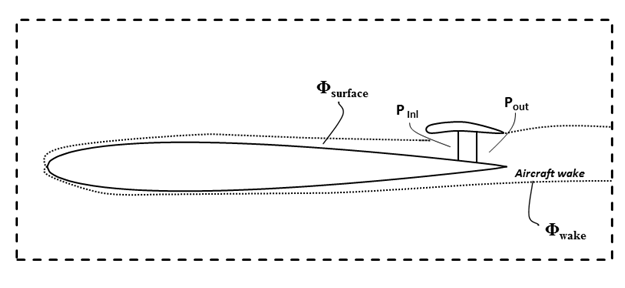
\includegraphics[width=120mm, height =60mm, clip=true]{Figure5_Control_Volume.png}
	\caption{Control volume of a notional hybrid wing body with embedded engines.}
	\label{Control_Volume}
	\end{figure}
	%%

According to \cite{Plas2007}, the general power balance equation for the podded case can be written as follows in equation \ref{Podded_Power_Balance}:

   \begin{equation}FV_\infty = D_{p}V_\infty + D_{i} V_\infty + W\dot{h}\label{Podded_Power_Balance}\end{equation}%

Where F is the net thrust of the propulsor and $D_i$ and $D_p$ are the induced and parasite drag as defined traditionally.  The equation for the BLI case can be written by \ref{BLI_Power_Balance} \cite{Plas2007}:

   \begin{equation}F^\prime V_\infty = D_p V_\infty - f_{BLI}\Phi_{wake} + D_{i} V_\infty + W\dot{h^\prime}\label{BLI_Power_Balance}\end{equation}%

Here the primes denote the BLI case, so the terms are differently than the podded case when denoted with a prime.  The $f_{BLI}$ term is the fraction of the trailing edge kinetic energy defect which is ingested into the propulsor.  The thing to note from equation \ref{BLI_Power_Balance} is that the primary consequence of the ingestion of the boundary layer is a reduction in the net thrust required (or power required) to propel the aircraft by overcoming its drag.  One additional thing to note is that the formulation given by \cite{Plas2007} does not include the changes to the clean drag polar terms ($D_p$ and $D_i$) incurred by the presence of the nacelle and engine sucking on the upper surface of the vehicle.  These terms could just as easily be included in the power balance relation if the interference effect between the engine and vehicle aerodynamics were known.  Finally, the $F^\prime$ term is the net thrust in the BLI case.  This is different than the traditional definition as shown in equation \ref{BLI_Net_Thrust}:
 \begin{equation}F^\prime V_\infty = f_{BLI}K_{TE} + \iint_{out}{V_\infty}u^\prime d\dot{m}^\prime\label{BLI_Net_Thrust}\end{equation}%

Here the net thrust is divided into what is traditionally known as the "gross thrust" as shown in the second term on the right hand side of equation \ref{BLI_Net_Thrust}.  The other term is the BLI effect on the inlet which must be accounted for by either a reduced total inlet pressure or ram drag accounting.

It can be shown that the above equations can be quantified by the use of the integral properties described in section 2.4.  Equation \ref{DBLI} shows the relationship between the podded drag and the BLI drag including the terms reduced by the re-energization effect due to the presence of the embedded propulsor.  The calculation of the dissipation factors are done via relationships given by \cite{Drela2009} in his description of the ideal wake ingesting propulsor.  
    \begin{equation}D_{BLI} = D_{Podded}-\displaystyle\sum_{k}\frac{\Phi_{BLI}}{u_\infty} = D_{Podded} - \frac{1}{u_\infty}\Big(\frac{1}{2}\rho_e u_e^3 \hat{\theta^*}\Big(2/H^*-1\Big)\Big) \label{DBLI}\end{equation}
    Assuming no rate of climb and rearranging the terms yields a useful relationship given by equation~\ref{NetThrust}.  This equation establishes the relationship between the net thrust defined
    \begin{equation}D_{Podded} = F_g - \dot{m}u_\infty\Big(1-\frac{\rho_\infty u_\infty \theta_{eq}}{\dot{m}}\Big)+\frac{1}{2}\rho_e u_e^3 \hat{\theta^*}\Big(2/H*-1\Big)\label{NetThrust}\end{equation}
    traditionally and the \emph{podded} drag polar.  This is useful because it allows the conceptual designer to approximate BLI in the ideal case by book-keeping the effects with the net thrust only and using the existing vehicle drag polar in the vehicle model.  This is convenient and consistent with the way engine drag effects are typically book-kept, which is to say that throttle dependent drag effects are contained with the net thrust.  This equation shows that the propulsive power benefits of BLI essentially come from the magnitude of the momentum and kinetic energy areas.  Therefore, uncertainty in these parameters translates into uncertainty with regard to the ability of the propulsion system to achieve the required level of net thrust.

\subsection{Metrics of Performance:  Propulsive Efficiency and Power Saving Coefficient}

There are, of course, multiple ways in which the performance of the BLI propulsor can be evaluated in comparison to the podded configuration.  The ultimate description of this comparison is contained in total mission fuel burn, which is the true objective of interest, but is a much more complicated metric to derive since one needs to be able to map engine performance over a mission flight envelope as well as to determine the effect on the system weight of embedding the engine as opposed to mounting them on pylons.  For the engines themselves, then, it is useful to define some of the typical metrics of performance whose trends strongly effect the fuel burn performance.  These are the propulsive efficiency and power saving coefficient.  

\indent The propulsive efficiency is defined by equation \ref{Propulsive_Efficiency_General} and is the ratio of the useful work being done by the propulsor to the rate of production of kinetic energy by the engine \cite{Plas2007}.
   \begin{equation}\frac{\Big(Total Drag\Big)u_\infty}
			      {\displaystyle \iint{\frac{1}{2}\Delta\Big(u^2\Big)\rho u dA}}\label{Propulsive_Efficiency_General}\end{equation}%

The velocities here are evaluated at free-stream pressure.  The propulsive efficiency trend is typically a good indicator of the fuel burn rate such that maximizing the propulsive efficiency tends to minimize the fuel burn, although maximizing propulsive efficiency may have an effect on the total drag due to the nacelle interference drag.  If the effect of the nacelle interference drag is small, then the propulsive efficiency should be a good indicator \cite{Plas2007}.  The propulsive efficiency in the case of BLI can be represented by equation \ref{Propulsive_Efficiency_BLI} which is derived in \cite{Plas2007}.  
   \begin{equation}\eta_{prop} = \frac{\Big(1+\beta\Big)}
					{\displaystyle \frac{H^*}{2} + \beta\Big[1+\frac{u_j-u_\infty}{2u_\infty}\Big]}\label{Propulsive_Efficiency_BLI}\end{equation}%

A plot of this equation vs. the normalized jet velocity (second term in the denominator of equation \ref{Propulsive_Efficiency_BLI}) is shown in figure \ref{Propulsive_Efficiency_Plot} for different values $\beta$.  The trend is the same as with the normal definition of the propulsive efficnecy vs. normalized velocity, except that there is the presence of the BLI effect in the calculation.  As the level of BLI is increased, the propulsive efficiency increases, which provides the basic motivation for the concept.
	%%
	\begin{figure}[htpb]
	\centering
	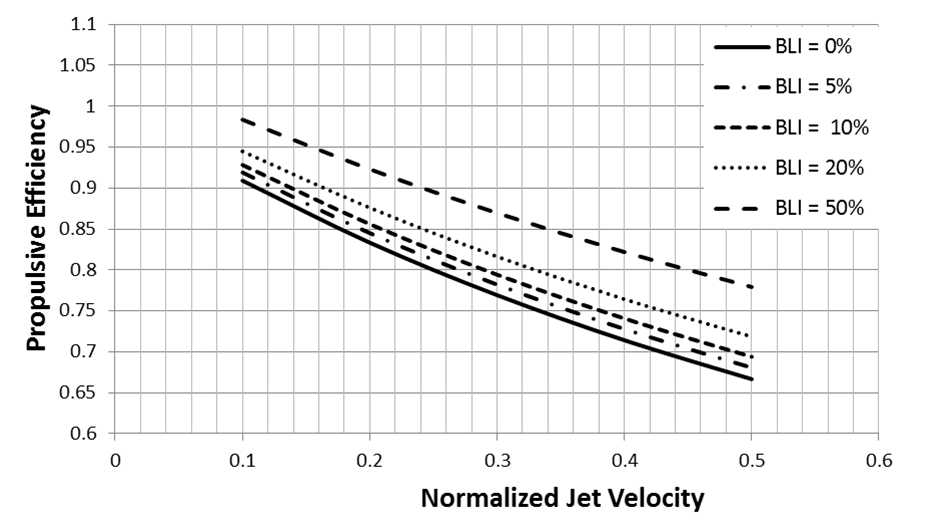
\includegraphics[width=120mm, height =70mm, trim=1mm 1mm 1mm 1mm, clip=true]{Figure6_Propulsive_Efficiency.png}
	\caption{Propulsive efficiency vs. normalized jet velocity for different values of \cite{Plas2007}.}
	\label{Propulsive_Efficiency_Plot}
	\end{figure}
	%%

Another relevant parameter for the evaluation of BLI is the power saving coefficient.  This will be denoted as PSC and is given by equation \ref{Power_Saving_Coefficient}.  It is the ratio of the difference between the power required to propel the aircraft for the BLI case and the podded case to the power required for the podded case.
\begin{equation}PSC = \frac{P_{ref} - P_{BLI}}
			              {P_{ref}}\label{Power_Saving_Coefficient}\end{equation}%

For a constant fan efficiency, the power saving coefficient should be directly related to the fuel burn of the engine.  Any BLI configuration should have a positive PSC in order to be considered a viable alternative to the podded case.

\subsection{Observations}

\fbox{
  \parbox{\textwidth}{
	Observation 1:  BLI performance benefits and engine sizing are functions of the airframe trailing kinetic energy defect.  

Observation 2:  Uncertainty in the aerodynamics of the vehicle propagates to uncertainty in the engine performance and efficiency.
	\vspace{5 mm}
	
Observation 3:  Ingesting more boundary layer improves the propulsive efficiency of the engine.
  }
}

\section{Airframe Aerodynamics and Boundary Layer}

The previous section discussed the power balance method and the metrics by which BLI performance can be estimated.  These turned out to be a function of the characteristics of the aerodynamics of the vehicle and specifically the boundary layer properties such as the momentum and kinetic energy thicknesses as well as the shape factors.  This section will discuss the methods by which system studies have estimated the inviscid airframe properties as well as the boundary layer properties needed for the performance analysis.

\subsection{Boundary Layer Characterization}
\indent There are a few general methods used to generate the airframe boundary layers.  The two primary methods for conceptual level system studies are summarized in Table \ref{Methods_Airframe}.  

\begin{table}[ht]
\caption{Summary of the two prominent methods for boundary layer characterization and their pros and cons for system level conceptual design studies with BLI.}
\centering
\begin{tabular}{cc}
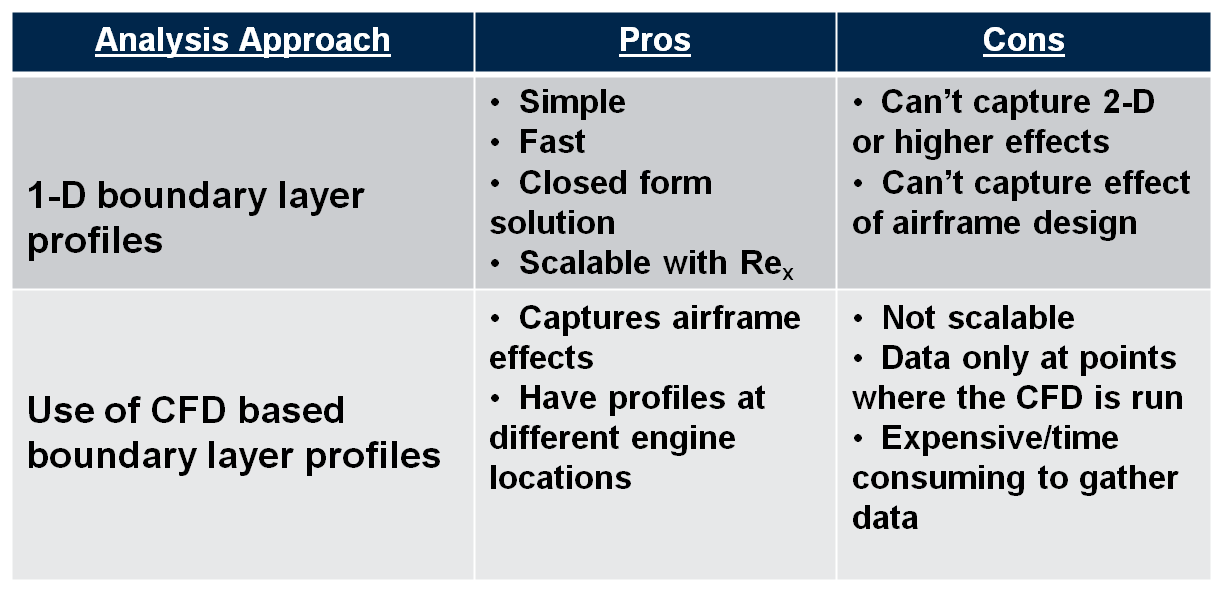
\includegraphics[width=120mm, height =70mm, clip=true]{Figure7_Methods_Airframe.png}
\end{tabular}
\label{Methods_Airframe}
\end{table}

Studies which use the first method include \cite{Sato2011} \cite{Plas2007}, and studies which use the second type of method include  \cite{Felder2011} \cite{Hardin2012} \cite{Kawai2006}.  The majority of system level studies avoid using CFD in the multi-disciplinary analysis loop, but rather assume that the boundary layers do not change much from the cruise point and simply use those profiles as a starting point.  From the first method, typical approaches are to assume a Coles wake profile or a $1/7^{th}$ power law profile which is typical of flat plate turbulent boundary layers.  Figure \ref{Boundary_Layer_Profiles} shows CFD data at the centerline of a Boeing HWB design \cite{Felder2011}
	%%
	\begin{figure}
	\centering
	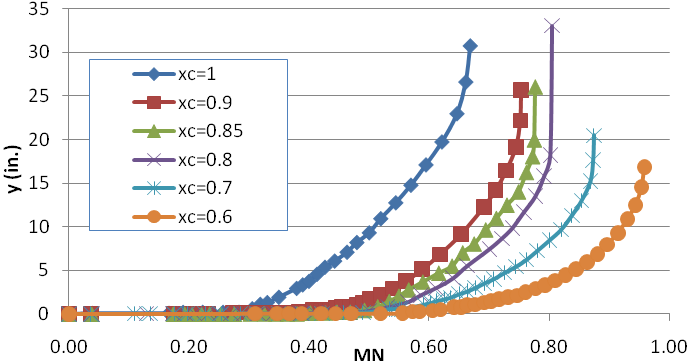
\includegraphics[width=120mm, height =70mm, clip=true]{Figure8_Boundary_Layers.png}
	\caption{Boundary layers profiles based on the Boeing HWB design and CFD analysis.  Plot of height above the airframe vs. axial Mach number. \cite{Fedler2011}}
	\label{Boundary_Layer_Profiles}
	\end{figure}
	%%
\subsection{Integral Properties}
\indent Based on this data, the boundary layer integral properties can be calculated along the airframe and the inviscid Mach number at the edge of the boundary layer can also be computed.  This data is shown in figure \ref{Integral_Properties} vs. the axial position along the aircraft centerline and shows that the properties grow as essentially the Reynolds length is increased.  The Mach number first increases along the suction side of the vehicle airfoil -- typically to a value that is transonic -- and then decreases on the aft end of the aircraft after about 60\% of the chord line due to the presence of the adverse static pressure gradient.
	%%
	\begin{figure}[htpb]
	\centering
	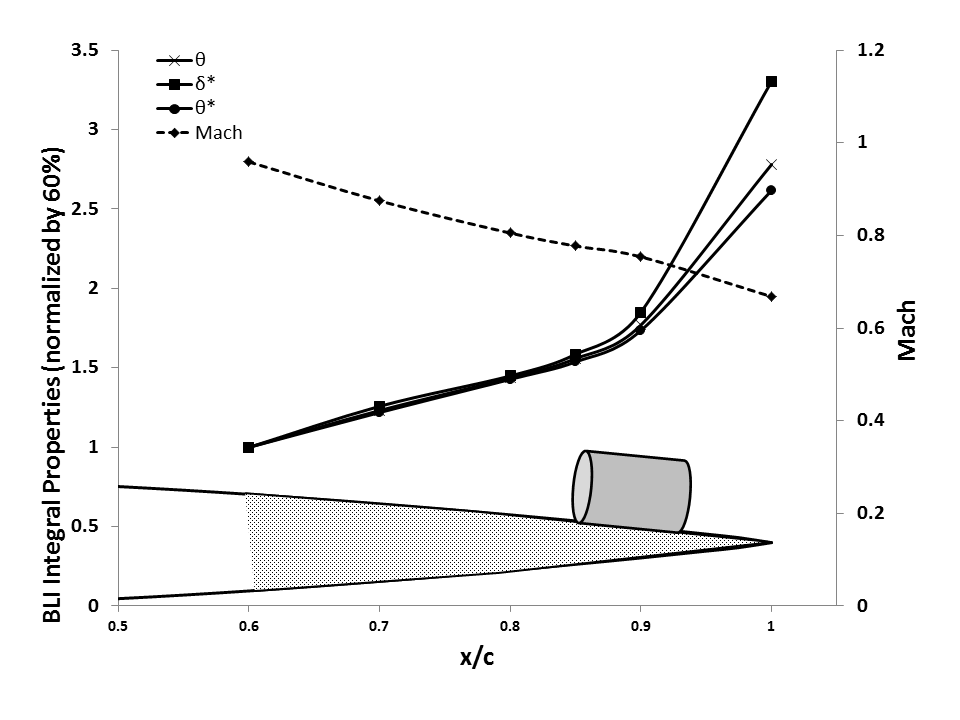
\includegraphics[width=120mm, height =70mm, clip=true]{Integral_Properties.png}
	\caption{Plot of Mach number, displacement, momentum, and kinetic energy defects vs. the axial length along the HWB centerline based on the Boeing CFD data.}
	\label{Integral_Properties}
	\end{figure}
	%%
Analyzing figure \ref{Integral_Properties} and the equations for the power balance of the aircraft, it is clear that the BLI benefit terms in the power balance equation, as well as in the propulsive efficiency equation are increased as the engine is moved farther aft, since the momentum and kinetic energy defects are increased as the length along the aircraft is increased.  It is also worth noting that the engines placed outboard of this position may be subject to a different pressure gradient, Reynolds length, and fundamentally different intake aerodynamics than the center line engine and will thus have differences in the installation BLI impacts on engine performance.  This has yet to be sufficiently addressed in the current literature.
\indent Another important point to be made is that for each flight condition, the angle of attack of the aircraft (typically set by lift and trim requirements) will have a strong impact on the flow entering the inlet.  It is thus necessary to map these boundary layer profiles as a function of this variable as well, which is not typically done.

\subsection{Observations}
\vspace{25pt}

\fbox{
  \parbox{\textwidth}{
Observation 4:  Existing system studies use either a simple 1-D boundary layer assumption or use tabular CFD data.  
\vspace{5 mm}
	
Observation 5:  The boundary layer varies as a function of flight condition, position on the airframe, and the angle of attack of the vehicle.
\vspace{5 mm}

  }
}

\section{BLI Inlet Modeling}
Figure \ref{Inlet_Diagram} outlines the various regions of the flow field leading up to the fan face of the embedded engine.  The pre-entry boundary layer region was described in the previous section along with the models that are typically employed for conceptual level studies.  Additionally, there is the "pre-compression" region which is described by Plas in \cite{PlasThesis}.  This is the region in which the streamtube is affected by the presence of the engine and the flow is compressed into the inlet capture area.  Flow that is not ingested into the engine passes over the external cowl region which may typically induce some drag due to wall pressure or shock wave generation.  
	%%
	\begin{figure}[htpb]
	\centering
	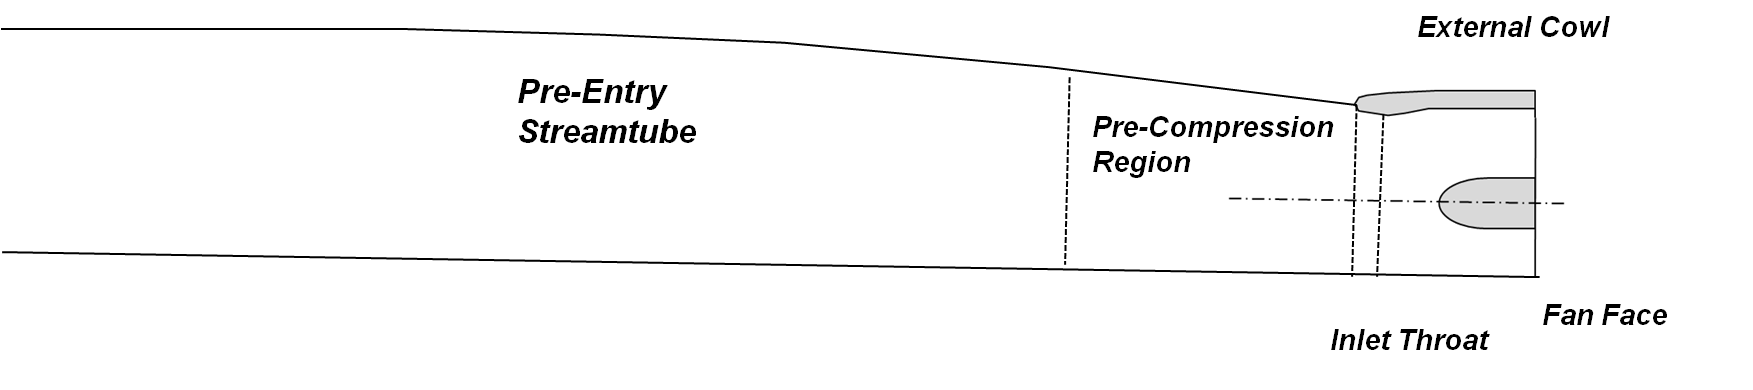
\includegraphics[width=160mm, height =45mm, clip=true]{Inlet_Diagram.png}
	\caption{Notional picture of the regions of the flow field before the fan face.}
	\label{Inlet_Diagram}
	\end{figure}
	%%
 Inside the inlet, the Mach number decreases as the flow is diffused inside the inlet until it reaches the fan face.  The fan face Mach number is typically a function of the fan design specific flow capability. 
\subsection{Pre-compression region}
\indent Most of the system studies ignore the effect of the pre-compression region.  This includes \cite{Felder2011} \cite{Hardin2012}.  Plas \cite{PlasThesis} included a model of the pre-compression region using the integral boundary layer theory and modeling the static pressure distribution as an exponential and linear distribution within the region.  This approach yields a physics-based method for determining the evolution of the boundary layer properties and thicknesses within the pre-compression region.  

\subsection{Inlet Sizing}
With the presence of the boundary layer, the mass flow entering the inlet can be described in terms of the displacement thickness as follows:
	\begin{equation}\frac{\dot{m}}
			              {\rho_eu_e} = \Big(A - b\delta^*\Big)
           \end{equation}%
Here b is the width of the inlet assuming a constant width over the height of the boundary layer.  If the displacement thickness is known along with the inlet capture area geometry, then the required capture height of the stream tube prior to pre-compression can be calculated to satisfy the mass flow demand of the engine.  This was the approach used by Plas \cite{PlasThesis} to size the inlet capture area.  Other authors including \cite{Felder2012} have simply ignored the pre-compression region and used the boundary layer profiles from the CFD data for the purpose of direct integration to determine the necessary capture height.
\indent With the capture height calculation, one can mass average the total pressures and temperatures from the wall to the capture height to determine an average recovery.  Felder showed representative curves of mass-averaged total properties vs. capture height which are reproduced in figure \ref{Total_Properties}.  This data is again based upon the Boeing HWB design CFD analysis.
	%%
	\begin{figure}[htpb]
	\centering
	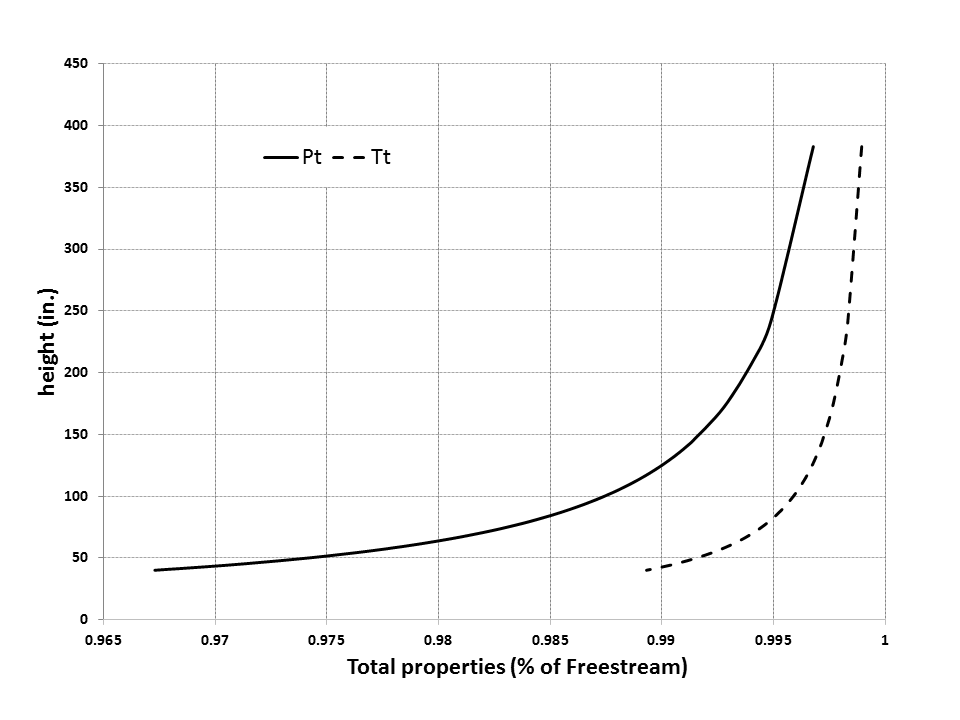
\includegraphics[width=130mm, height =100mm, clip=true, trim = 5mm 0mm 0mm 0mm]{Total_Properties.png}
	 \vspace{-25pt}
	\caption{Mass averaged total pressure and temperature prior to the pre-compression region for the Boeing HWB design.}
	\label{Total_Properties}
	\end{figure}
	%%
\subsection{Inlet Duct Recovery}
Finally, the last component of the aerodynamic analysis prior to the fan face is the performance of the inlet duct.  The necessary output of this analysis depends upon the fidelity of the fan model used.  If the fan model requires more detailed fan face profiles, then a higher fidelity analysis must be used.  If the fan model requires only a characterization of the "dirty" or distorted region, then a simple 1-D type analysis might suffice, such as the integral boundary layer method \cite{PlasThesis}.  By far the most common approach, however, is the use of a simple inlet recovery parameter or inlet efficiency as is used in standard cycle analysis techniques.  This means that the BLI losses are essentially passed as a lower mass averaged pressure recovery to the standard fan analysis.  This approach is used in \cite{Felder2011} \cite{Sato2011} \cite{Hardin2012} \cite{Nickol2009}  with various values assumed for the pressure loss, which tends to have a significant impact on BLI performance.

\subsection{Observations}
\fbox{
  \parbox{\textwidth}{
Observation 6:  The performance of the inlet is a function of the incoming airframe flow field, the pre-compression region, and the duct design; thus there is a coupling between the airframe boundary layer (and therefore flight conditions, angle of attack, etc.), the ingested streamtube height, and the inlet performance.   
	\vspace{5 mm}
	
Observation 7:  As the streamtube height is decreased, the average total pressure and temperature recovery is reduced.  This implies that using more, smaller engines, will lead to worse average inlet performance to be traded against the BLI propulsive efficiency benefits.

  }
}

\section{Fan Modeling}
\indent At the conceptual, system study level, the fan modeling approach taken is typically a simple efficiency hit.  This approach was used in \cite{Felder2011} \cite{Sato2011} \cite{Hardin2012} \cite{Nickol2009}  .  Although simple, it does provide a basic parametric way to understand the impact of the fan performance relative to the BLI propulsive efficiency benefits to understand technology targets for a BLI fan design.  Table \ref{Fan_Efficiency_Assumptions} shows the differences in assumptions used for the fan efficiency for some of the important system studies mentioned earlier.  It is common to assume that the efficiency penalty will be small, however recent work conducted by Pratt and Whitney \cite{Florea2013} shows that there is a likely efficiency penalty relative to a clean fan on the order of 0-1.5\%.  

\begin{table}[ht]
\caption{Fan efficiency assumption used for several system studies.}
\centering
\begin{tabular}{cc}
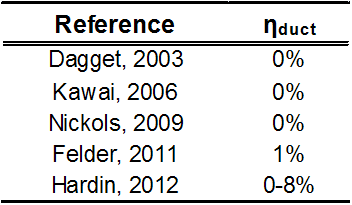
\includegraphics[width=60mm, height =40mm, clip=true, trim = 0mm 0mm 0mm 0mm]{Fan_Efficiency_Assumptions.png}
\end{tabular}
\label{Fan_Efficiency_Assumptions}
\end{table}

As discussed previously, Plas \cite{Plas2007} conducted a study on 3 different levels of modeling fidelity for a ducted fan.  For brevity, the details of each model will not be discussed here, but rather some of the key conclusions from the study will be summarized and some observations will be made that are relevant for the current work.

\subsection{Parallel Compressor Model}
The basics of the parallel compressor model is to model the fan component as separate compressors with different total pressure, axial velocity, and mass flow but with the same speed and characteristic line (PR vs. corrected mass flow).  This model is useful because it creates a coupling between the nature of the distorted flow field (i.e. the magnitude of the $P_t$ deficit), the fan design via the characteristic, and the final efficiency and pressure ratio.  Figure \ref{PC_Figure} shows a simple illustration of the model on a fan map of PR vs. corrected mass flow.  
	%%
	\begin{figure}[htpb]
	\centering
	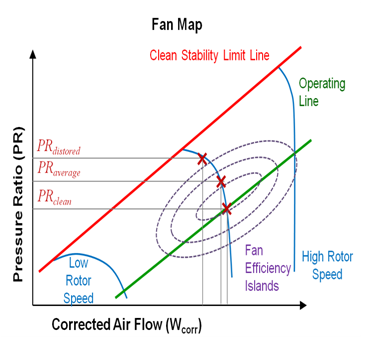
\includegraphics[width=90mm, height =60mm, clip=true, trim = 0mm 0mm 0mm 0mm]{PC_Figure.png}
	\caption{Illustration of the parallel compressor model on a notional fan map.}
	\label{PC_Figure}
	\end{figure}
	%%

\indent The parallel compressor model used by Plas is essentially the simplest possible model because it employs a "2-segment" approach, with one dirty and one clean sector.  It is possible to include more sectors should the flow coming into the fan be proven to be more complex \cite{Greitzer1993}.  The parallel compressor model has been successfully used for performance prediction in the gas turbine industry and can also be used for operability prediction in certain cases.  Recent work has shown it's effectiveness for different types of inlet distortion in comparison to experimental rig data \cite{Cousins2011}.

\subsection{Higher Fidelity Models}
\indent Plas additionally employed two other higher fidelity models:  an integral boundary layer method and a 3-D body force model.  Both models showed differences from the PC approach ranging from 10-40\%, and more importantly, these approaches show the importance of the distortion attenuation and nozzle losses in determining the performance of the unducted propulsor.  This study shows that the attenuation must be modeled in some way and viewed parametrically, and also that the fidelity of simpler models can have significant impact on the viability of a BLI system.  The difficulty with the 3-D models is that it requires computationally expensive high-fidelity physics calculations, meaning that it is difficult to make the approach parametric for large design space explorations.  Additionally, a designer would ideally like to have a map for off-design performance calculations, so for each design a separate 3-D map would need to be created.  This makes the 3-D approaches somewhat less appealing in the context of conceptual design.  

\subsection{Fan Distortion}
As shown by the parallel compressor model, the performance of the fan can be impacted by the presence of inlet distortion.  However, perhaps more significantly is the impact on the fan stall margin.  Figure \ref{PC_Figure} shows that the dirty sector of the distortion is closer to the stall margin because the PR is more and the mass flow less in that region.  SAE ARP1420 \cite{ARP1420} provides parameters that can describe a total pressure distortion for an inlet aerodynamic interface plane (AIP).  Figure \ref{Circumferential_Distortion} illustrates a circumferential variation in the total pressure at a particular radial location for a single-per-rev type distortion (one continuous dirty sector).
	%%
	\begin{figure}[htpb]
	\centering
	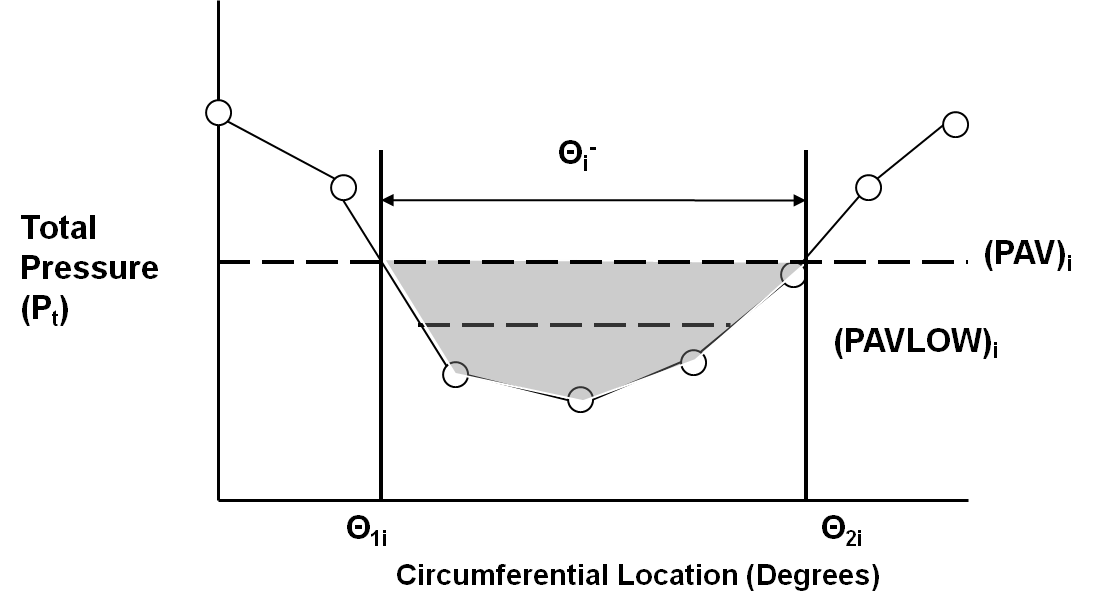
\includegraphics[width=110mm, height =70mm, clip=true, trim = 0mm 0mm 0mm 0mm]{Circumferential_Distortion.png}
	\caption{Typical circumeferential distortion distribution for a single-per-rev type distortion profile at the $i_{th}$ radial ring.}
	\label{Circumferential_Distortion}
	\end{figure}
	%%
The circumferential distortion prescribed by ARP1420 guidelines is given by equation \ref{Circum_Descriptor}, where the terms in the equations are defined by equations \ref{Paverage} and \ref{PaverageLow}.
\begin{equation}\Big(\frac{\Delta PC}
			          {P}\Big)_i = \Big(\frac{PAV-PAVLOW}
							  {PAV}\Big)_i
\label{Circum_Descriptor}\end{equation}%

\begin{equation}PAV_i = \frac{1}
 				      {360} \int_0^{360}{P(\theta)_i d\theta}
\label{Paverage}\end{equation}%

\begin{equation}PAVLOW_i = \frac{1}
                                                 {\theta_i^-}\int_{\theta_{1i}}^{\theta_{2i}}{P(\theta)_i d\theta}
\label{PaverageLow}\end{equation}%

Finally, the radial distortion prescribed by ARP1420 is shown in equation \ref{Radial_Descriptor}, where PFAV is given by equation \ref{PFAV} and is the averaged over the i radial rings.
\begin{equation}
	\Big(\frac{\Delta PR}
		    {P}\Big)_i = \frac{PFAV-PAV_i}
					{PFAV}
\label{Radial_Descriptor}\end{equation}%

\begin{equation}
	PFAV = \frac{1}
		         {N} \sum\limits_{i=1}^{N} PAV_i
\label{PFAV}\end{equation}%

Analyzing the above equations, one point seems salient, namely that the lower the average pressure, the higher the circumferential and radial distortion descriptors.  This means that if the stall margin reduction is correlated with the descriptor, as is typically done, then lowering the heights of the inlet using smaller inlet heights and more engines should tend to move the fan closer to the stall line.  Thus, there may be, depending on the fan characteristic and quality of the fan inlet flow, a point where smaller engines are simply limited by the operability constraint. 

\indent To date there have been no significant efforts to incorporate the operability concerns into the boundary layer ingestion modeling approaches at the conceptual level.  Perhaps the closest attempt to do so was done by Rodriguez for the case of the 3 engine BWB configuration.  His approach was to simply use distortion descriptors as a constraint on the inlet design, so that the optimization would maintain sufficiently low distortion while maximizing efficiency.  This may, in fact, prove useful in the preliminary design phase of the inlet, but remains difficult at the conceptual level when the general propulsion system layout has yet to be determined and is perhaps even more difficult for engine designers who may need to make decision before such high fidelity modeling is available.
\vspace{25pt}

\fbox{
  \parbox{\textwidth}{
Observation 7:  None of the system studies to date have considered operability within the context of engine sizing for boundary layer ingesting engines.
\vspace{5 mm}
	
Observation 8:  The stall margin of the fan is decreased as the height of the inlet capture area is decreased due to the increased circumferentially and radially averaged pressure distortion descriptors.
\vspace{5 mm}

Observation 9:  Adding additional stall margin has the effect of decreasing fan efficiency.
  }
}

\section{BLI Cycle Analysis and Propulsion System Design Requirements}
	As discussed previously, the typical tool set for the engine designer at the conceptual level is engine thermodynamic cycle analysis.  The point of the cycle analysis at the conceptual level is to establish an engine aerothermodynamic cycle which can satisfy all of the requirements of the engine while minimizing operational costs such as fuel burn.  In the early years of cycle analysis, cycle trade studies were the primary tools for conducting the parametric engine cycle design studies, while the advent of the modern computer and computer aided design has enabled the integration of other aspects of the design process such as engine flowpath, aircraft mission and cost analyses.  Additionally, modern design techniques enable broad trade space exploration and optimization within the context of these computational models.  Along the same lines, engine and airframe integration, especially in the military realm, has had a similar history with increasing tendency towards integrated design processes to facilitate increasing design knowledge early in the design phase to eliminate costly design changes in the later phases.  This section will look at the latest cycle analysis techniques and requirements specified in the case of boundary layer ingestion inlet integration and cycle analysis.  

\subsection{The Subsonic Airframe Integration Process}
\indent Since this thesis primarily will focus on BLI for reduction in civil aviation fuel burn, it is worth looking at the current inlet and engine integration processes and requirements which are typical and to also consider how the BLI concept might change this paradigm.  Firstly, civil transports of the kind to be considered for BLI will spend the vast majority of their time at the cruise condition.  For that reason, cruise fuel burn is typically considered the metric of interest in most studies.  However, of course it is worth mentioning that cruise does not take place at a fixed altitude, but rather a range of altitudes and Mach numbers during flight, with the vehicle lift, angle of attack, and pressure distribution changing as fuel is burned.  Typically the engine is sized for some value of thrust at the top-of-climb condition where mass flow is a maximum.  Additionally, there is typically some maximum specified turbine inlet temperature at take-off where the engine is running at its hottest, and the engine has to be able to supply the necessary thrust to achieve a particular take-off field length and climb rate.  The point is that there are a large range of operating conditions from take-off through climb, cruise, and descent which the inlet must supply sufficiently clean air for the propulsion system to supply the necessary thrust power to fly the vehicle.  At each of these flight conditions, there is a different interaction between the airframe boundary layer and the engine than at the cruise condition.  This difference will have an impact on performance through the BLI effects discussed in previous sections, but also on the ability of the propulsion system to meet the requirements.  Uncertainty in these interactions could lead to mistakes in design choices or fundamentally overestimated benefit of the technology, leading to a totally inferior aircraft relative to the state of the art podded engines.  Such mistakes could have catastrophic consequences considering the modern economic climate.

\subsubsection{Subsonic Flow Incidence Requirements}
\indent Although the inlet and airframe integration process is somewhat less tedious than for the military case, since civil transports clearly do not have as many critical maneuvers as military planes, the point still remains that there are multiple conditions in which the geometric orientation of the airframe causes potential problems for an engine inlet.  Perhaps most important among these are conditions such as take-off, climb, and landing where the vehicle and engine might be at an increased angle of incidence relative to the free-stream.  The inlet mass flow ratio is the parameter that best describes the approaching flow and is given by equation \ref{Mass_Flow_Ratio}.
\begin{equation}
	\frac{A_o}
	        {A_i} = \frac{\Big(\dot{m}_2 \sqrt{\theta_2}/\delta_2\Big)\Big(\delta_2/\delta_o\Big)}{\Big(\dot{m}\sqrt{\theta}/\delta A\Big)_o\Big(A_i\Big)} = \frac{\Big(\dot{m}\sqrt{\theta}/\delta\Big)_2\Big(\pi_d\Big)}{\Big(\dot{m}\sqrt{\theta}/\delta A\Big)_o\Big(A_i\Big)}
			       {}
\label{Mass_Flow_Ratio}\end{equation}%
\indent Oates states that:  "For subsonic inlets, the numerical value of $A_o/A_i$ is a direct indication of the general incidence of the flow approaching the inlet.  A value of unity means that the inlet is capturing its projection in the freestream and the stagnation point will occur at the inlet highlight for level flight.  A value less than unity indicates flow is prediffusing in the freestream, such that an outward flow incidence occurs; this is generally the case for cruise flight speeds.  Conversely,$A_o/A_i$ will exceed unity at low flight speeds and moderate to high power settings, such that an inward flow incidence develops with the stagnation point on the outer portion of the lip."  Furthermore, other flight conditions in which flow incidence is induced produce a velocity component normal to the freestream on top of the basic mass flow effect.   Figure \ref{Inlet_Incidence_Schematic} illustrates these issues \cite{Oates1989} for different flight conditions.
	%%
	\begin{figure}[htpb]
	\centering
	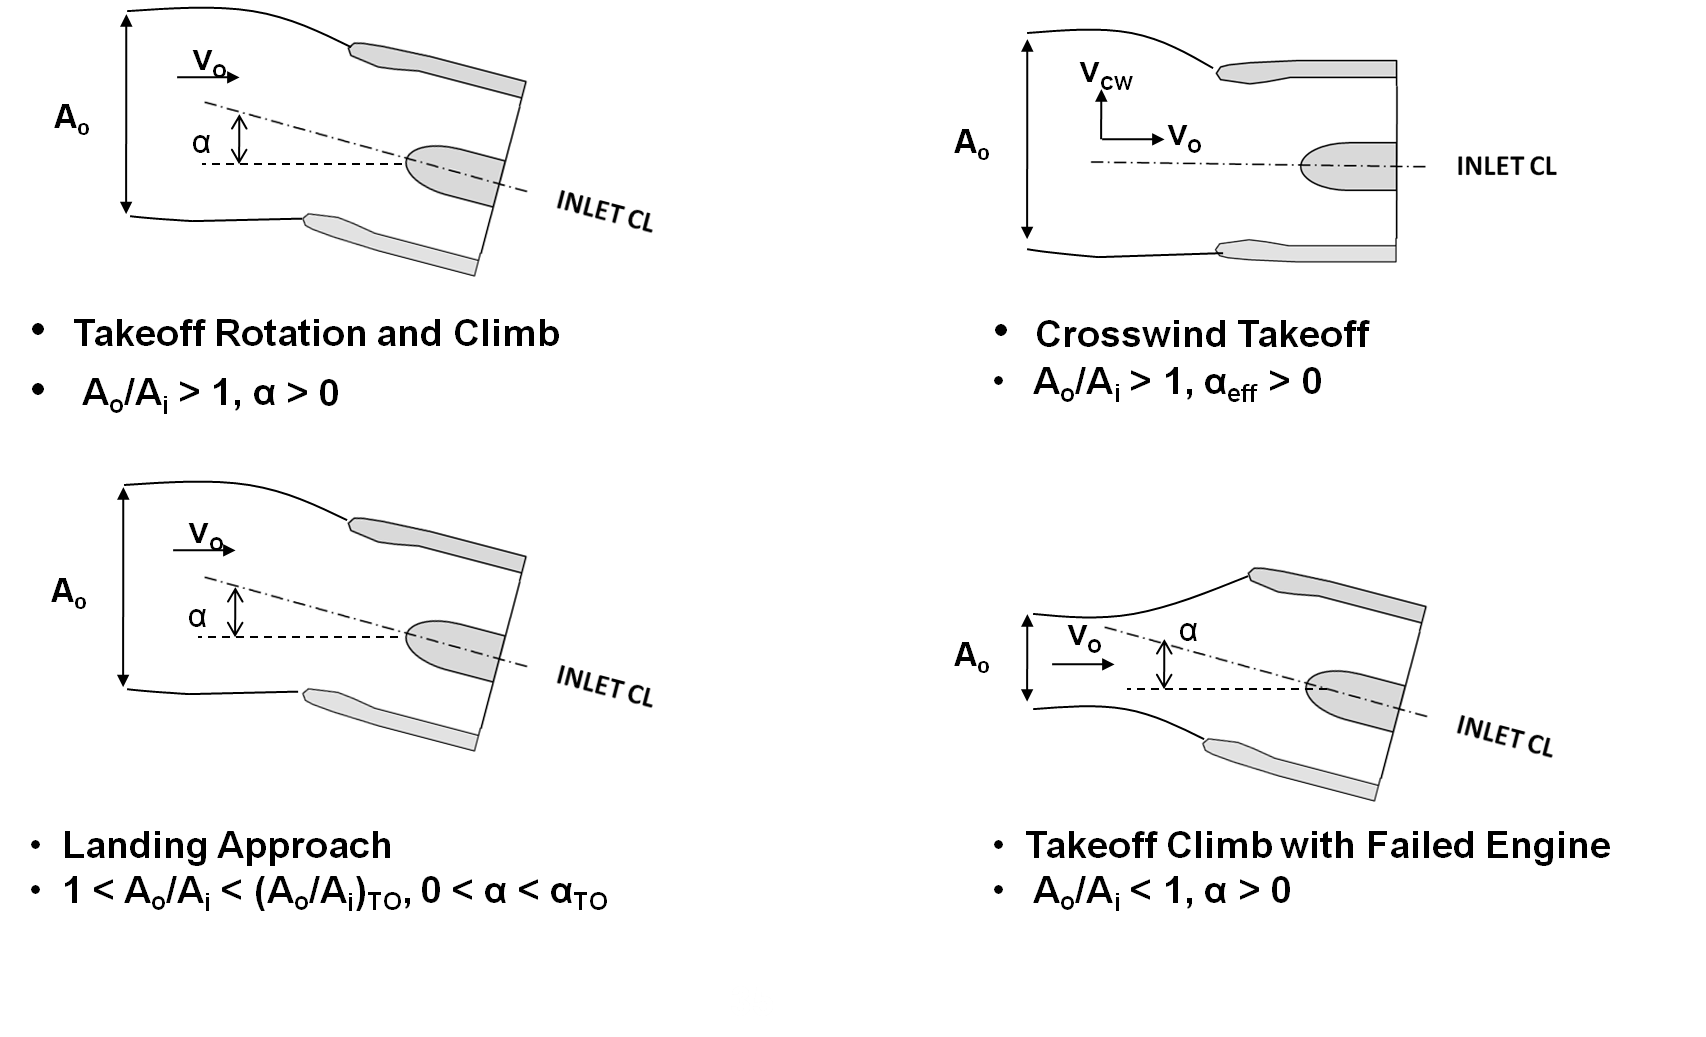
\includegraphics[width=140mm, height =85mm, clip=true, trim = 0mm 0mm 0mm 0mm]{Inlet_Incidence_Conditions.png}
	\caption{Notional inlet diagrams showing different conditions for which there are high inlet incidence angles \cite{Oates1989}}
	\label{Circumferential_Distortion}
	\end{figure}
	%%
For each of these flight conditions, there is a danger that the flow could separate as it passes over the lower inlet lip, thus producing potentially unacceptable distortion levels.  The engine must still be able to supply relatively low distortion flow to the inlet such that the engine maintains thrust and does not surge.  Furthermore, this condition must be satisfied over a range of free-stream Mach numbers, since the aircraft is accelerating during climb and deccelerating during landing.  Typical engine incidence requirements are shown plotted vs. freestream Mach number in figure \ref{Alpha_Incidence_Requirements}.  

	%%
	\begin{figure}[htpb]
	\centering
	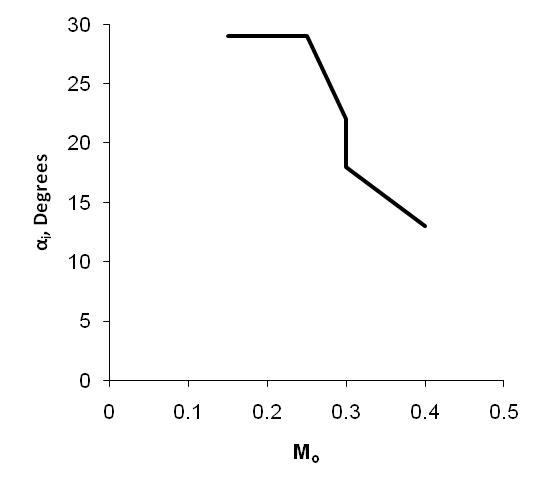
\includegraphics[width=120mm, height =85mm, clip=true, trim = 0mm 0mm 0mm 0mm]{Alpha_Incidence_Requirements.png}
	\caption{Notional inlet incidence angle requirements vs. freestream Mach number \cite{Oates1989}}
	\label{Alpha_Incidence_Requirements}
	\end{figure}
	%%

Finally, it is worth discussing the take-off with engine out condition.  This is critical since the engine is operating at peak temperature during take-off meaning that a failure is likely to happen at that condition since the majority of the damage to the components occurs there.  If an engine goes out, the ingested mass flow ratio is significantly less than unity since the engine is windmilling.  At this condition, the external cowl can produce significant drag due to the flow accelerating rapidly over the cowl lip.  The remaining operating engines must be able to overcome this drag on it's own with sufficient climb rate.  

\subsection{BLI as a Paradigm Shift}
\indent With the preceeding understanding of the limiting flight conditions for typical subsonic inlet integration, it is now necessary to consider how the above might change if there is some base level of distortion being ingested into the engine.  Firstly, the fundamental difference between the embedded engine and the podded engine is that the danger due to separation is coming from the airframe itself rather than the inlet lip.  This means that the level of distortion is inherently greater and the consequence of flow separation potentially greater as well.  It is logical to speculate then, that the BLI engines will struggle to meet the vehicle incidence requirements.  Indeed, the angle of attack envelope of the vehicle may need to be limited by the distortion limits of the engine as a function of Mach number.  All of this has hitherto been unaddressed in the analysis literature, even with computational fluids tools, much less in the system study literature.  Since these concerns may ultimately limit the possible engine configurations and also impact the cycle designs, there is a need to integrate these design conditions into conceptual design cycle analysis framework to at minimum understand their impact.  

\indent Another level of complexity generated by the boundary layer ingesting engine has to do with the placement of the engines on the airframe.  First, the placement of each engine (or array of engines in the case of distributed propulsion) is now a design variable, although it is certainly subject to key constraints such as stability and control and similar practical concerns.  Furthermore, since preceeding sections have substantiated that having smaller engines distributed across the airframe suction surface potentially offers higher BLI propulsive efficiency gains, there is a problem of having different airframe-engine interference for different sets of engines.  For instance, if there are three engines such as in the work of Rodriguez \cite{RodriguezThesis}, then the centerline engine may have quite different inlet flow properties -- primarily boundary layer thickness -- and subsequent performance impacts.  As a corollary to this, Rodriguez showed that a proper inlet aerodynamic optimization might yield different inlet designs and slighty different inlet orientation for the inboard and outboard.  This would then mean that the recoveries and distortion levels between the engines are different even though each engine is subject to the same operability constraints.  To date, one system study has looked at the possibility of quantifying the impact of this \cite{Sato2011} effect in terms of the BLI propulsive efficiency benefit.  This study determined that if one does not consider the effect in the fuel burn calculations, then BLI benefit is rather significantly over predicted (which for BLI could mean 1 or 2\%).  Another computational fluids study \cite{Kim2012} which showed this effect was done for the Boeing N2B design, in which the boundary layer thickness was found to differ by as much as a factor or two between inboard and outboard propulsors. 
\subsection{MDP Analysis}

\indent The preceeding section established that although cruise is the primary condition where the performance of the engine is most consequential in terms of fuel burn, that there are several other "off-design" conditions where the engine thrust capability must be sufficient and might therefore be candidates for inclusion into the engine cycle selection process.  The traditional engine design process has been performed at a single design point to set the cycle.  Performance at other operating conditions is then evaluated in off-design analysis.  Though this standard approach provides a good basis for understanding the trends of gas turbine performance, it does not provide a practical approach for a designer to match an engine and performance requirements for a particular airframe.  

\indent Schutte \cite{SchutteThesis} designed and analyzed a methodology called simultaneous "multi-point design", in which modern computational tools are used in an engine sizing process which simultaneously satisfies engine requirements and constraints at multiple flight conditions.  This is done by linking engine "On-Design" and "Off-Design" within a modified Newton-Raphson solver to satisfy the thrust constraints at all conditions.  The process is necessary because it allows the formation of an engine cycle design space where each candidate cycle design is inherently feasible so long as the technology assumptions are physically achievable.  This eliminates needless manual iteration between the single point engine "On-Design" solutions and other off-design solutions.  The MDP concept is shown graphically in \ref{MDP_System_of_Equations}.  The design points are linked via the simultaneous solution of a system of equations.

	%%
	\begin{figure}[htpb]
	\centering
	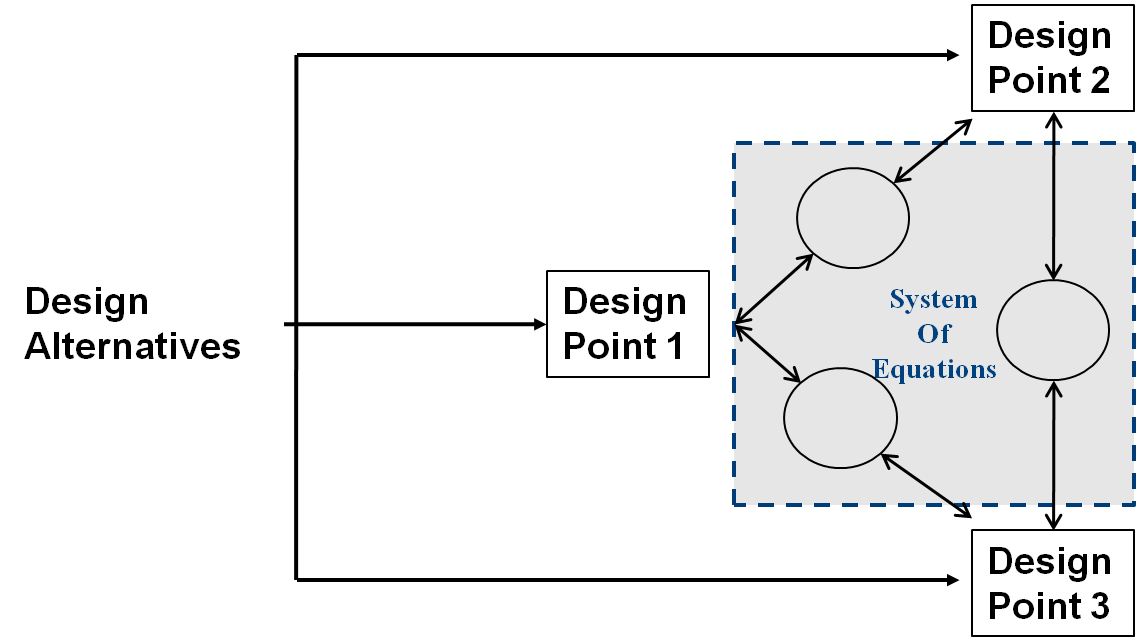
\includegraphics[width=110mm, height =70mm, clip=true, trim = 0mm 0mm 0mm 0mm]{MDP_System_of_Equations.png}
	\caption{Simultaneous multi-design point cycle analysis equation setup \cite{SchutteThesis}}
	\label{MDP_System_of_Equations}
	\end{figure}
	%%

\subsection{BLI Cycle Analysis Approaches}
\indent To date, the cycle analysis requirements specified in the BLI engine design literature have been of the traditional style.  Typically a sizing point is set, such as top-of-climb, and the engine size is based on the required mass flow to achieve the engine thrust at that point.  A few authors have additionally included analyses of the off-design points to check for sufficient sea-level static and take-off thrusts \cite{Felder2011} \cite{Sato2011}.  Most of the higher fidelity studies do not touch the engine models, with perhaps the exception of Rodriguez who did vary the engine bypass ratio independently and used the cruise point as the engine sizing point \cite{RodriguezThesis} \cite{Rodriguez2009}.  Thus, no author has previously handled the issue of simultaneous satisfaction of the requirements discussed in the previous section above, the method by which this might take place, and the implications of this procedure on the resulting engine sizes.  A significant part of this work will be to address this issue directly.

\subsection{Observations}
\vspace{25pt}

\fbox{
  \parbox{\textwidth}{
Observation 10:  Boundary layer ingesting studies to date have only done single design point cycle analysis for engine design.
\vspace{5 mm}
	
Observation 11:  Subsonic inlets are constrained by incidence requirements to maintain quality engine airflow during critical flight conditions.  Boundary layer ingestion may further constrain the possible angle of incidence over which the engine can operate without encountering surge.
\vspace{5 mm}

  }
}	

	\chapter{A General Method for BLI Propulsion System Design, Integration, and Analysis}
\section{Methodology Development}
\subsection{MDP Cycle Analysis}
\subsection{Requirements for a BLI Sizing Method}
\subsection{Methodology and Justification}
\section{BLI Modeling Phase}
The history of the analysis of boundary layer ingesting engines, much as the history of any analysis, is littered with varying levels of modeling fidelity and assumptions with often quite disparate results INSERT REFERENCE HERE.  The complicated nature of the question -- viscous and turbulent airframe-propulsion interaction -- often lends itself to convenient simplications for the sake of expediency in order to draw some initial conclusion about potential net benefits and viable configurations.  Once such decisions have been made, engineers are free to move on to the difficult work of determining the validity of the assumptions and analysis via higher order toolsets such as modern Navier-Stokes codes and the like.  This is all very typical of a usual design process, in which conceptual design begins with some crude assumption and is refined by later analysis and optimization.  However, the point of this thesis is to try to get closer to a feasible answer -- at least for the basic propulsion system cycle design and sizing -- before the aerodynamicists embark on refining the assumptions that went into making that decision.  Furthermore, it is intended to guide the aerodynamicist and experimentalist in appropriately directing finite resources for their efforts in the most productive directions (correct flight conditions, configurations, initial geometry, etc), and providing sufficient data back to the propulsion engineer in an iterative process which eventually converges on a solution.  It is with this basic project in mind that research question 1 is formulated and stated simply as follows:
\vspace{25pt}
\vspace{5mm}
\fbox{
  \parbox{\textwidth}{
Research Question 1:  What are the minimum requirements for conceptual level modeling of a boundary layer ingesting cycle model in order to reasonably construct the architecture and cycle design space of a BLI propulsion system?
\vspace{5 mm}
  }
}
\vspace{5mm}

Note that the question asks for the "minimum" modeling requirements for conceptual design.  In a sense, this is asking "what can we get away with" or "what is good enough" at the conceptual level, since obviously the best case scenario is to build a complicated fluid dynamics model, allow it to run on an infinitely powerful computer, and come back with an answer.  Unfortunately, no such computer exists and even if it did, we'd have to ask about exactly which design we are modeling to start.

In attempting to answer this question, we first take on some components of the answer as being trivial; one needs a reasonable engine cycle model to begin with, as well as thermodynamic component models for the constituent machinery and ducting;  one also needs some approximation of the vehicle flow field at the points where it interacts with the engine and a total clean vehicle drag which translates to a thrust requirement.  These are the first few blocks of the "BLI modeling phase" and it is somewhat obvious that they must be known to complete any analysis of the system.  

The component of the question which is far more interesting, however, is in quantifying the interaction between the flow field and propulsion system and its impact on system performance.  These interactions can broadly be classified into 3 regimes: power balance (or thrust balance), turbomachinery performance and efficiency, and engine stability.  The first two have been looked at by almost every author on the subject, while the latter has been studied by some component designers, aerodynamic engineers, and a few others INSERT REFERENCE HERE.  Stability, though it is certainly a dominant concern among technologists, planners INSERT REFERENCE HERE, and experimentalists INSERT REFERENCE HERE, has tended to take a "back seat" at the cycle analysis level, in part because it is a difficult subject to analyze, but also because it is often assumed that modern aerodynamic methods will solve the problem after the fact INSERT REFERENCE HERE.  For this reason, we will begin the analysis by ignoring the stall margin question and returning to it later to analyze this dubious partitioning of the problem.

The analysis will also be separated into two different operational modes: engine on-design and off-design.  On-design is the analysis which typically sets the size of the engine, while off-design is any operational condition which deviates from those conditions, including variations in flight Mach number, altitude, or throttle setting ("part power").  On-design analysis essentially sets the level of thrust production and efficiency that the system is capable of providing, while the off-design analysis determines the variation of those quantities over a range of operating conditions.  The ultimate system fuel burn which results is actually a function of both on-design and off-design analysis, since the mission analysis which is typical requires performance over a wide variety of flight conditions.  It is thus necessary to consider both modes of operation, but we will begin, perhaps logically, with the subject of engine on-design analysis.

\subsection{On Design Analysis with BLI}

Engine on-design cycle analysis is the standard term for thermodynamic analysis which determines the size, mass flow (therefore thrust capability), and efficiency of an engine.  The engine design process usually begins with this type of analysis, however the final selection of the design is usually determined by off-design performance (to be discussed later) over the entire aircraft mission during the cycle selection process INSERT REFERENCE HERE.  This analysis is often carried out at a single design point in the simplest case, though it is difficult to often determine the proper design point where a significant portion of cycle choices at that point will yield feasible off-design performance.  Schutte INSERT REFERENCE HERE showed how modern cycle analysis tools and techniques can be used to implement a multi-design point approach (MDP), the purpose of which is to "ensure the feasbility of all cycle designs for a particular application".  This principle ought to -- and, in fact, does -- apply in the case of BLI, however the theoretical and academic work which implements BLI on-design analysis has largely ignored the issue of off-design performance and proceeds with determining performance differences at a nominal cruise point.  For BLI systems, especially those applied to the HWB aircraft concept, the typical flight condition assumed for the analysis is in excess of Mach 0.7, though typically closer to a 0.8-0.85 range.  The usual design point in these studies is a "top of climb" -- or maximum mass flow -- condition where corrected thrust required is largest.

The process for assessing the benefit of BLI at the design point chosen typically comes down to finding some means of translating the impact of the ingestion of the boundary layer on the propulsive efficiency.  The two equations shown below from Smith and Plas exhibit this mode of thinking about the problem.  Both equations represent the propulsive efficiency of a BLI ingesting propulsor in terms of some measure of the level of boundary layer ingested ( D/T for Smith, $\beta$ for Plas) and in terms of parameters describing the character of the wake or boundary layer being ingested.  The equations are slightly different since Smith and Plas are analyzing different conceptual configurations and propulsor designs and because of modeling assumptions.  However, the core objective remains the same:  to describe the benefit gained from BLI as a function of the amount of wake ingested and boundary layer parameters.  Fundamentally, the results from this analysis are similar:  ingesting more boundary layer provides a bigger benefit.  Other methods of analysis have been used, which involve translating the boundary layer velocity profile into an equivalent "ram drag" reduction -- sometimes called the "ram drag approach" -- and has yielded similar results.  None of these approaches are specific to engine on-design, as they could in principle be used to quantify off-design performance benefit as well, but they are typically applied at the engine design point in the sizing and cycle design analysis.
  
   \begin{equation}\eta_{prop} = \frac{2}{\displaystyle\frac{V_j}{V_o} + 1 - \frac{D}{T}\Big[\displaystyle\frac{V_j}{V_o} -1 + R (1-K)\Big]}  \label{Smith_Propulsive_Efficiency}\end{equation}%

   \begin{equation}\eta_{prop} = \frac{\Big(1+\beta\Big)}
					{\displaystyle \frac{H^*}{2} + \beta\Big[1+\frac{u_j-u_\infty}{2u_\infty}\Big]}\label{Plas_Propulsive_Efficiency}\end{equation}%

\vspace{15pt}
This standard observation from the BLI literature is therefore formulated as follows:

\vspace{1pt}
\vspace{5mm}
\fbox{
  \parbox{\textwidth}{
\textbf{Observation 1}:  The performance benefit of boundary layer ingestion systems is generally a function of the ratio of the ingested drag to the uningested drag -- or net thrust required.
\vspace{5 mm}
  }
}
\vspace{5mm}

The obvious question which arises from this observation pertains to which factors determine the percentage of BLI ingested in relation to the net thrust.  This question obviously relates to the manner in which one calculates the percentage of BLI ingested.  
Smith \cite{Smith1993} considers the case of a wake ingesting propeller and gives an equation for the amount of BLI ingested in terms of the momentum thickness as shown in equation \ref{Smith_Ingested_Drag}.
   \begin{equation}D = \rho V_o^2 \theta \label{Smith_Ingested_Drag}\end{equation}%
This equation is essentially a momentum balance approach which attempts to quantify the change in the net thrust of the vehicle due to wake ingestion as a function of the momentum deficit.  Here the density, velocity, and wake momentum deficit are defined at the entry of the propeller "actuator" disk.  This equation is the starting point for the development of equation \ref{Smith_Propulsive_Efficiency} and the D/T contained in that equation results from the form of equation \ref{Smith_Ingested_Drag}.  The ingested drag from \ref{Smith_Ingested_Drag} is seen as contingent upon the size of the momentum deficit in the wake.  Note that momentum deficit here is defined as a momentum area rather than a thickness as sometimes defined for 1-D boundary layers.  This means that this parameter is really a function of both the general momentum thickness of the wake and also the extent of the wake which is actually ingested.  The combined deficit integral over the control volume entrance then gives the final value of the wake momentum area deficit.  The point is that both the character of the wake and the amount of wake ingested has an influence on the amount of drag ingested.

Smith proceeds with a parametric approach with regard to the ratio of ingested drag to thrust and looks at the effect of this parameter on the propulsive efficiency as a function of the thrust loading coefficient $(C_{th})$.  He concludes his analysis by stating the following:  
\begin{quote}
 \textit{...for best efficiency the propulsor should be positioned and sized to ingest as much wake fluid as possible (increase D/T), but after that, making it still larger does not pay off in propulsive efficiency and would have other adverse effects such as increased weight.}
\end{quote}
This analysis assumes that at a certain point, the propulsor will be large enough to ingest the majority of the wake and therefore any attempt to make it larger would have diminishing returns due to weight increase.  For configurations such as those where the wake is distributed along a very large span such as that for the HWB aircraft, this analysis may break down and there may be additional gains from making the propulsors even larger or distributing a very large number of smaller propulsors across the upper surface.  In any case, the operative principle which is established here is that there is an important relationship between the sizing and positioning of the engine and the amount of boundary layer that can be ingested.  

Plas \cite{Plas2007} gives a slightly different expression for the calculation of the ingested drag percentage as show in equation \ref{Plas_Ingested_Drag}.

\begin{equation}D_w =  \rho u^2 \Big(\frac{u}{u_o}\Big)^{H_{avg}}\theta_o b\label{Plas_Ingested_Drag}\end{equation}%

In this case, the ingested drag is calculated based on a dissipation or energy based approach originally defined by Drela \cite{Drela2009}, where the ingested drag is essentially the dissipation coefficient divided by the free-stream velocity to convert it into the amount of equivalent thrust saved by the ingestion.  This equation is similar to equation \ref{Smith_Ingested_Drag} except that it is using the kinetic energy deficit rather than the momentum deficit though it calculates this by approximating the kinetic energy shape factor from the average shape factor.  

The variable "b" here is a term representing the "span" of the ingested boundary layer.  This variable essentially translates the 1-D kinetic energy thickness into an equivalent ingested area defect and therefore produces the correct thrust/drag modification.  The details of whether to use momentum or energy based approches can be discussed, but again the main point to be seen here is that benefit of wake ingestion ultimately relies upon some character of the boundary layer profile (momentum or KE deficit) and the extent or span of the ingested streamtube in relation to the overall required thrust of the system.  It is worth mentioning that there are many other studies essentially corroborating this basic principle and focusing on the relationship between the amount of BLI ingested and efficiency increase.  Observation 2 is therefore formulated as follows:

\vspace{1pt}
\vspace{5mm}
\fbox{
  \parbox{\textwidth}{
\textbf{Observation 2}:  The ratio of uningested drag to net thrust depends on both the value of the boundary layer defect properties and the span of the boundary layer ingested by the engine stream-tube.
\vspace{5 mm}
  }
}
\vspace{5mm}

\subsection{Off-Design Analysis}
\subsection{Hypothesis 1}

\subsection{Stall Margin and Stall Constraint}
\subsection{Hypothesis 2}

\section{Architecture Integration Phase}
\subsection{Integration Issues and Observations}
\subsection{Hypothesis 3}
\subsection{Design Possibilities}
\subsection{Hypothesis 4}

\section{Vehicle Matching Phase}
\subsection{General Criteria for BLI Sizing Condition}
\subsection{Hypothesis 5}
\subsection{Vehicle Matching Methodology}
\subsection{Integration with MDP Analysis}

	

	\chapter{BLI Modeling Phase}
	In the previous chapter, the overall BLIPSS methodology was developed and hypotheses 1 and 2 were made based on observations from past literature and additional theoretical analysis.  This chapter will demonstrate the BLI modeling phase, as outlined in Chapter 3, for a canonical design problem involving a hybrid wing body vehicle with boundary layer ingesting turbofan engines.  The chapter will proceed according to the outline of the BLI modeling phase and the BLI component modeling process defined in Chapter 3.  Furthermore, experiments intended to validate hypotheses 1 and 2 will be defined and conducted in order to justify the need for each of the components of the method and to determine which physical effects are relatively important for this canonical problem.  
	
	The chapter will first outline the baseline vehicle design and geometry and thrust requirements for the propulsion system.  The baseline propulsion system will also be specified and defined in detail for purposes of comparison with the BLI designs.  The BLI modeling components for the propulsion system will be defined in detail and verification/validation data will be provided to substantiate the models.  Experiments 1 and 2 will be defined and the results will then be shown to draw conclusions in relation to hypotheses 1 and 2.  		
	
	\section{Baseline Design}
		%% Should EDS stuff go here?  Description of the modeling environment?
		\subsection{Baseline Vehicle}
			The baseline vehicle used here is very similar to the Boeing N2A-EXTE design INSERT REFERENCE NASA LANGLEY.  The vehicle is intended to carry 300 passengers and would therefore be a future potential replacement for a Boeing 777 (double aisle) type airplane.  Some overall assumed parameters for the vehicle which are relevant to the BLI problem are shown below.\\ 
			
			\begin{table}[htp]			
					\centering
					\renewcommand{\arraystretch}{1.5}% Spread rows out...
					\begin{tabular}{|>{\centering\arraybackslash}m{4cm}| >{\centering\arraybackslash}m{3cm}|}
						\hline
						Parameter & Value \\
						\hline
						Gross Weight & 536,282 lbs \\
						Wing Span & 240 ft \\
						Max Fuel &  197,000 lbs \\
						Cruise Mach & 0.84 \\
						Initial Cruise Alt & 35,917 ft \\
						Final Cruise Alt & 43,000 ft \\
						Initial Cruise L/D & 21.6 \\
						Final Cruise L/D & 20.0 \\
						SLS Thrust/Engine & 72,400 \\
						Design Range & 7530 nm \\
						Payload & 64,000 lbs \\
						\hline
					\end{tabular}
					\captionof{table}{Table showing key design parameters for the baseline HWB vehicle.}
					\label{Baseline_Design_Table}	
			\end{table}
			
		
				\begin{figure}[htp]
					\centering
					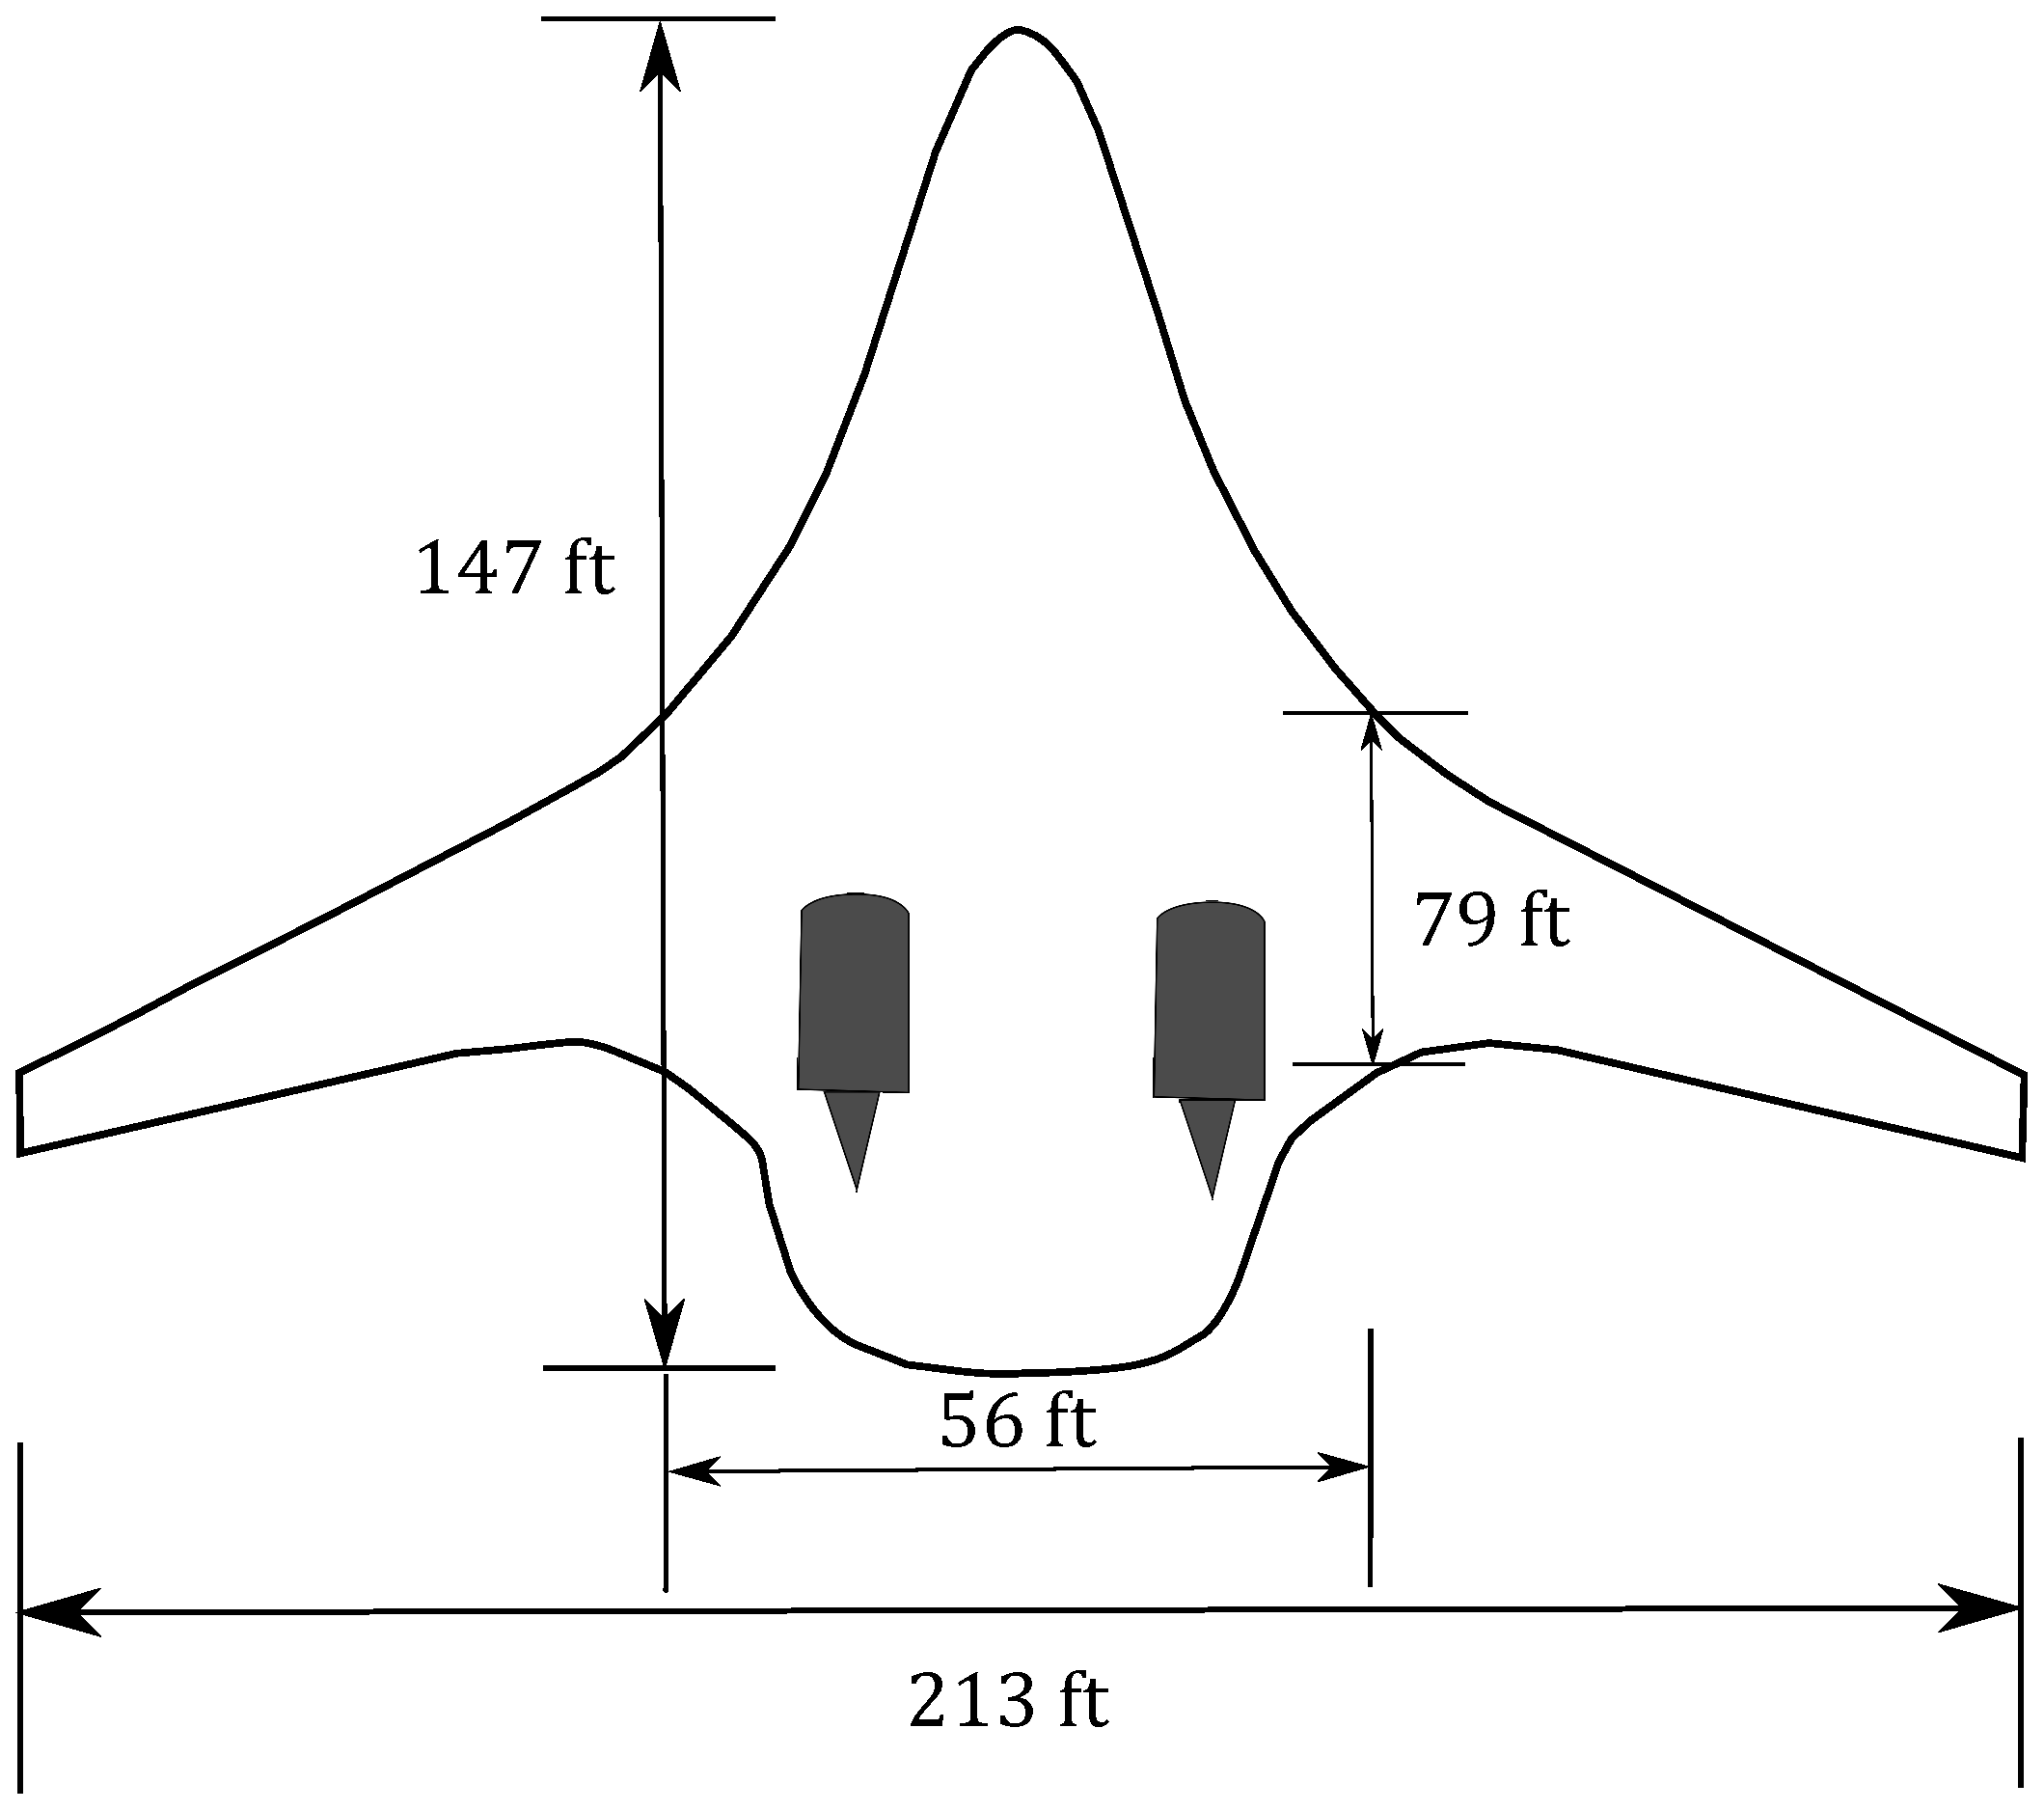
\includegraphics[scale = 0.3]{HWB_Dimensions.eps}
					\captionof{figure}{HWB baseline key design dimensions.}
					\label{Baseline_Design_Table}
				\end{figure}
				

												
			\subsubsection{Available Vehicle Boundary Layer}
			
			
	\section{Baseline Engine}
	\section{BLI Modeling}
		\subsection{Airframe Model}
		\subsection{Power Balance and Drag Book-keeping}
		\subsection{Inlet Model}
		\subsection{Fan Model}
			\subsubsection{General Model Architecture and Algorithm}
			
	\section{Experiment 1 Results}
	
	\subsection{Flight Condition Variation}
	
	\subsubsection{Design Mach Number}
	
	\subsubsection{Design AoA Impact}
	
	\subsection{BLI Design Space Variation}
	
	\subsubsection{Influence of Inlet Aperture Shape}
	
	\subsubsection{Influence of Engine Number}
	
	\subsection{Off-Design Variation}
	
	\subsubsection{Mass Flow Variation}
	
	\subsubsection{Influence of the Pre-entry zone}
	
	\subsubsection{Influence of Flight Condition}
	
	\subsubsection{Impact On MDP Sizing}
	
	\section{Stall Margin Test Experimental Setup}
	
	\subsection{Stall Margin Criteria and Allowables}
	
	\section{Experiment 2 Results}
	
	\section{Summary and Conclusions}

	\chapter{Architecture Integration Phase}

\section{Implementation of Methodology on HWB Vehicle}
\section{Wake Correction Method}
\section{Experiment 3 Results}
\section{Experiment 4 Results}

	\chapter{Vehicle Matching Phase}
\section{Methodology for Flight Condition Determination}
\section{Initial MDP Setup}
\subsection{Effect of BLI On MDP Results}
\section{Methodology Implementation on Baseline Vehicle}
\subsection{Baseline Vehicle Requirements}
\subsection{Algorithm Description}
\section{Experiment 5 Results}
\subsection{Baseline Thrust and Stall Margin}
\subsection{Initial BLI Design and Critical Flight Conditions}
\subsection{BLI Re-Design}

	%%
	\begin{figure}[p]
	\centering
	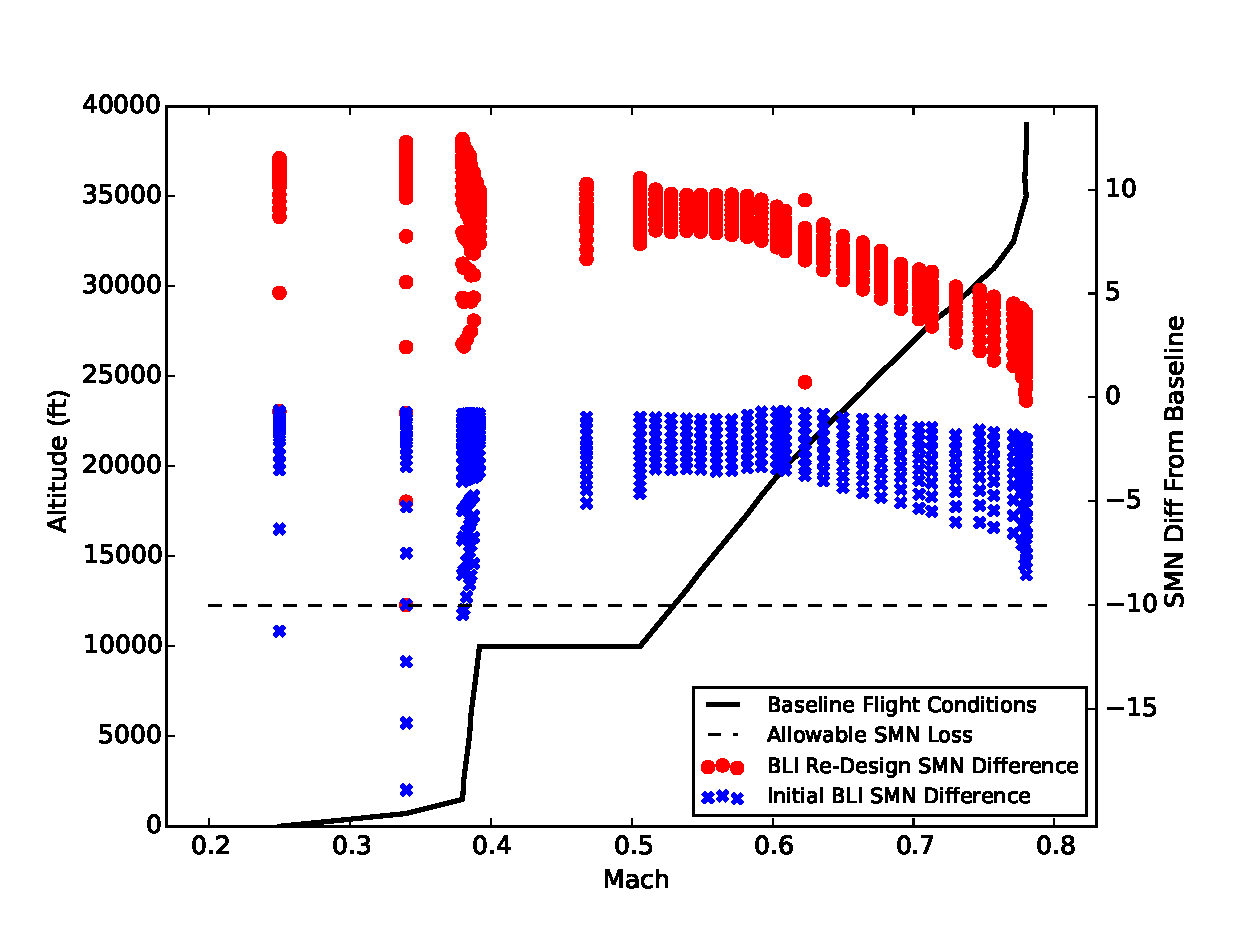
\includegraphics[width=0.8\textwidth]{plot6-5.eps}
	\caption{Angle of attack performance variation for different fidelity models.}
	\label{alpha_sweeps}
	\end{figure}
	%%

\subsection{Impact of BLI Design Variables on Critical Flight Conditions}
\subsection{Impact of Cycle Design Variables on Critical Flight Conditions}
\subsection{Variable Area Nozzle Results}


	\chapter{Summary and Conclusions}

\nocite{*}
%% We need this since this file doesn't ACTUALLY \cite anything...
%%
 
\begin{postliminary}
\references
\end{postliminary}


\end{document}
